\documentclass[11pt]{article}
\usepackage[margin=1in]{geometry}
\usepackage[T1]{fontenc}
\usepackage[utf8]{inputenc}
\usepackage{lmodern}
\usepackage{amsmath,amssymb,amsthm,mathtools,bm}
\usepackage{booktabs,enumitem,graphicx,xcolor,tikz}
\usetikzlibrary{arrows.meta,positioning,calc,fit,backgrounds}
\usepackage{microtype}
\PassOptionsToPackage{hyphens}{url}
\usepackage[hidelinks]{hyperref}
\hypersetup{pdftitle={An FPRAS for Cell-Bounded Contingency Tables},pdfauthor={OpenAI},pdfsubject={Approximate counting with binary capacities}}
\ifdefined\pdfinfoomitdate\pdfinfoomitdate=1\fi
\ifdefined\pdftrailerid\pdftrailerid{}\fi
\ifdefined\pdfsuppressptexinfo\pdfsuppressptexinfo=15\fi
\newtheorem{theorem}{Theorem}[section]
\newtheorem{lemma}[theorem]{Lemma}
\newtheorem{proposition}[theorem]{Proposition}
\newtheorem{corollary}[theorem]{Corollary}
\theoremstyle{definition}
\newtheorem{definition}[theorem]{Definition}
\theoremstyle{remark}
\newtheorem{remark}[theorem]{Remark}
\DeclareMathOperator{\dist}{dist}
\DeclareMathOperator{\Var}{Var}
\DeclareMathOperator{\Cov}{Cov}
\DeclareMathOperator{\TV}{TV}
\let\epsilon\varepsilon
\newcommand{\E}{\mathbb E}
\renewcommand{\P}{\mathbb P}
\setlist{itemsep=2pt,topsep=5pt}
\allowdisplaybreaks[2]
\title{An FPRAS for Cell-Bounded Contingency Tables}
\author{OpenAI}
\date{September 24, 2026}
\begin{document}
\maketitle
\begin{abstract}
We give a fully polynomial randomized approximation scheme for counting
nonnegative integer matrices with prescribed row sums, column sums, and
individual entry bounds. Both dimensions vary, all numerical data are encoded
in binary, and zero bounds are allowed. The algorithm uses only unbiased random
bits and has a polynomial bound on its bit operations on every execution.
\end{abstract}
\section{Introduction}\label{sec:introduction}
A cell-bounded contingency table is a nonnegative integer matrix whose
row sums, column sums, and individual entry bounds are prescribed.
For positive integers $m,n$, margins
$r\in\mathbb Z_{\ge0}^m$ and $c\in\mathbb Z_{\ge0}^n$ with equal total,
and bounds $b\in\mathbb Z_{\ge0}^{m\times n}$, write
\begin{equation}\label{eq:feasible-set}
\begin{aligned}
 \Omega(r,c,b)&=\left\{X\in\mathbb Z_{\ge0}^{m\times n}:
 \sum_{j=1}^n X_{ij}=r_i,\quad
 \sum_{i=1}^m X_{ij}=c_j,\quad X_{ij}\le b_{ij}\right\},\\
 Z(r,c,b)&=|\Omega(r,c,b)|.
\end{aligned}
\end{equation}
Each table is counted once. In particular, $b_{ij}=0$ forbids an entry;
no positivity condition is imposed on the support or margins.
Our concern is the binary encoding model, in which a capacity can be
exponentially larger than its description. Both $m$ and $n$ are part of
the input.

\begin{theorem}\label{thm:main}
There is one randomized algorithm with the following guarantee. Given
$(r,c,b)$ as above and rational $\varepsilon,\delta\in(0,1)$, it outputs
a nonnegative rational $\widehat Z$ such that
\[
 \P\bigl((1-\varepsilon)Z(r,c,b)\le \widehat Z
                  \le(1+\varepsilon)Z(r,c,b)\bigr)\ge1-\delta.
\]
If $\Omega(r,c,b)$ is empty, the output is zero on every execution.
The algorithm uses independent unbiased bits, and one fixed polynomial
in $L$, $\varepsilon^{-1}$, and $\log(\delta^{-1})$ bounds its total bit
operations on every execution, where $L$ is the total binary input
length, including the accuracy parameters. No counting or sampling
oracle is required.
\end{theorem}

The theorem allows arbitrary cell bounds and margins without a fixed
number of rows or columns, a lower bound on positive capacities, or a
density or balance assumption. Its running-time guarantee includes
preprocessing, random-bit generation, rational arithmetic, and output,
even on executions in the failure event. The polynomial bounds in the
proof are deliberately generous; the result is a uniform complexity
guarantee rather than a practical running-time estimate.

\subsection{History and significance}
The enumeration of fixed-margin arrays has long been studied in
statistics and combinatorics; Diaconis and Gangolli~\cite{DG1995}
survey its applications and exact and approximate methods.
Ordinary contingency tables are a special case of
\eqref{eq:feasible-set}, since the margins imply
$X_{ij}\le\min\{r_i,c_j\}$. Even their exact enumeration is difficult:
Dyer, Kannan, and Mount~\cite[Theorem~1]{DKM1997} proved
$\#\mathrm P$-completeness for tables with only two rows.
Approximate counting can nevertheless be efficient under much broader
conditions than exact counting.

For ordinary tables, Dyer, Kannan, and Mount~\cite{DKM1997}
developed geometric sampling and counting methods for sufficiently
large margins. Morris~\cite{Morris2002} weakened the required margin
bounds by refining the expanded-polytope and rounding argument.
Dyer and Greenhill~\cite{DG2000} gave polynomial-time approximate
counting and sampling for arbitrary two-row margins. Cryan and
Dyer~\cite{CD2003} obtained an FPRAS for any fixed number of rows by
combining dynamic programming and volume estimation; Dyer~\cite{Dyer2003}
subsequently improved the fixed-row algorithm using dynamic programming.
Gopalan, Klivans, Meka, \v{S}tefankovi\v{c}, Vempala, and
Vigoda~\cite[Theorem~1.3]{GKM2011} later gave a deterministic FPTAS
for a fixed number of rows.
These results already permit binary-encoded margins. Their restrictions
concern the number of rows or the sizes of the margins, rather than a
unary encoding convention.

Individual caps connect the problem to several other counting models.
When all caps are zero or one, a table is a subgraph of the allowed
bipartite graph with prescribed vertex degrees. Jerrum, Sinclair, and
Vigoda~\cite[Corollary~8.1]{JSV2004} give an FPRAS for this entire
special case as a consequence of their permanent algorithm; all-one
margins give perfect matchings. Bez\'akov\'a, Bhatnagar, and
Vigoda~\cite{BBV2007} developed a direct annealing algorithm for
binary tables, also allowing arbitrary forbidden cells.
More generally, capped tables are
integer flows in a bipartite network. Cryan, Dyer, and
Randall~\cite{CDR2010} gave an FPRAS for integral flows with sufficiently
large tight capacities, and for cell-bounded tables with a fixed number
of rows and arbitrary positive margins and caps. They identified
unrestricted approximation as an open problem in their 2010 paper.
Their tight-capacity reduction and maximum-capacity spanning-tree
representation are direct antecedents of our large-cell construction.
Here a forest and soft constraints accommodate arbitrary mixtures of
small and large bounds, with both dimensions variable and zero bounds
permitted.

Convex optimization gives a complementary family of estimates.
Barvinok~\cite[Theorem~1.3]{Barvinok2009} bounds ordinary weighted
table counts, including forbidden cells, within a factor
$N^{O(m+n)}$, where $N$ is the total margin. Barvinok, Luria,
Samorodnitsky, and Yong~\cite{BLSY2010} obtain randomized relative
approximations with complexity $N^{O(\log N)}$ for specified
smooth-margin classes. This scale is quasipolynomial in the numerical
total, rather than in its binary length. Br\"and\'en, Leake, and
Pak~\cite[Theorem~2.1]{BLP2021} give capacity bounds for arbitrary
individual caps, with explicit multiplicative factors depending on
the margins and dimensions. Their bounds extend earlier estimates
using Lorentzian polynomials. A subsequent preprint of September 30,
2026, by Leake and Mohammadi Yekta~\cite[Theorems~1.1 and~1.3]{LMY2026}
extends capacity-based estimates to finite nonnegative integer fibers
of totally unimodular systems, retaining an explicit multiplicative
factor depending on the system's dimensions and right-hand side.
Theorem~\ref{thm:main} supplies
any requested relative tolerance in polynomial binary time, without
a smoothness assumption.

The geometric problem here is to count all integer points of a
transportation polytope. These need not all be vertices: the
$2\times2$ tables with every margin equal to two form a segment
with three integer points and two vertices. Guo and
Jerrum~\cite[Proposition~4.2]{GJ2023} give an FPRAS for the vertices
of promised $0/1$ polytopes $\{x:0\le Ax\le1\}$ defined by network
matrices; this unit-bound vertex result has a different scope.

Counting also provides approximate sampling through the
self-reduction principle of Jerrum, Valiant, and
Vazirani~\cite[Theorem~6.3]{JVV1986}. Section~\ref{sec:flows}
implements this principle by bisecting cell intervals, with exact
feasibility tests at every branch. For an explicitly given directed
multigraph with finite integer arc bounds and prescribed vertex
balances, it yields both an FPRAS for integer arc-value vectors and
a sampler that always returns a feasible vector when one exists.
The latter has total-variation error at most $\tau$ and an
all-execution cost polynomial in the input length and $\tau^{-1}$.
A separate companion~\cite[Theorem~1.1]{OpenAIExactTables2026}
proves exact uniform sampling in polynomial expected bit time for
ordinary tables with arbitrary margins and no input cell bounds or
forbidden positions. Its bounded approximate sampler has cost
polynomial in the input length and the number of accuracy bits. Those stronger sampling
guarantees concern the uncapped setting; the flow consequence here
has the total-variation and cost bounds just stated.


\subsection{From tables to weighted transversals}
The proof separates numerical size from combinatorial complexity.
Large binary bounds cannot be expanded into that many binary choices.
We instead sum over large coordinates through a weighted completion
problem, and expand only coordinates with polynomially bounded ranges.
The resulting finite-state argument must preserve one unit of mass per
table despite the multiplicities introduced by this expansion.

\paragraph{Large entries and two views of a small entry.}
Flow feasibility first tightens each cell to its attainable interval.
Subtract its minimum, so that the new endpoints are $0$ and $b_s$;
each endpoint is attained by some feasible table. Remove zero-width
cells and separate the remaining cells at a polynomial threshold $W$.
In the bipartite graph of large cells, choose a maximum-capacity
spanning forest and one root in each component. The large cells outside
the forest are free coordinates. Once their values and the contributions
of small cells to each incident margin have been specified, leaf
elimination uniquely determines the tree entries from the nonroot
margin equations.

For a small cell $s$, temporarily allow two counts $x_s,y_s$ between
$0$ and $b_s$: its row contribution is $x_s$, and its column
contribution is $b_s-y_s$. The views agree when $x_s+y_s=b_s$.
Writing $p=\sum_{s\text{ small}}b_s$, we also consider unbalanced
profiles satisfying only $\sum_s(x_s+y_s)=p$. Extending the weights
to these profiles supplies the auxiliary states and algebraic tests
used below. For every such
profile, sum over the free large entries in their integer intervals.
Penalize the resulting deviations from root margins and violations of
tree-cell bounds by a nonnegative quantity $D$. This penalty vanishes
exactly when those remaining constraints hold. A maximum-capacity
forest bounds its slopes in normalized free coordinates independently
of the numerical large capacities.

For a polynomially bounded integer $H$, let $h_j(x,y)$ be the sum of
$2^{-jD/H}$ over these free assignments, for $0\le j\le H$, and
let $C(j)$ be the sum of $h_j$ over balanced small profiles. Thus
$C(0)$ is an explicit product of interval sizes. Every feasible table
contributes one to $C(H)$, while invalid completions contribute
additional positive mass. Log-concavity of each tree-coordinate marginal,
together with its attainable endpoints, controls violations close to
a tree boundary; exponential decay controls more distant violations.
This proves $Z\le C(H)\le(1+\epsilon/32)Z$. The use of scaled free
coordinates and soft constraints builds on the geometric table methods
of Dyer, Kannan, and Mount and Morris~\cite{DKM1997,Morris2002}.

\paragraph{Binary encodings and two extensions of their weights.}
Replace a small cell of bound $b_s$ by $b_s$ labeled pairs, each
containing a row element and a column element. There are $p$ pairs
altogether. A \emph{transversal} selects one element from each pair.
Its selected row and column counts give a balanced profile $(x,y)$.
The number of transversals with that profile is
$\prod_s\binom{b_s}{x_s}$, so assigning each the weight
$h_j(x,y)/\prod_s\binom{b_s}{x_s}$ gives mass $h_j(x,y)$ to that
profile and total mass $C(j)$ to all transversals.

The transport argument uses an enlarged chain that also permits $p$-element sets
with one empty pair and one full pair. Such a state has \emph{defect
type} $(i,l)$ when pair $i$ is empty and pair $l$ is full.
Two factorial formulas extend the transversal weights to positive
weights $f_j$ and $\widetilde f_j$ on all $p$-element sets. They
agree on transversals and are within a polynomial factor of each other
on the permitted defect types. Their algebraic roles differ. For $f_j$,
matrices of weights obtained by omitting two elements from a fixed
$(p+2)$-element set have at most one positive eigenvalue. For
$\widetilde f_j$, the corresponding statement holds when adding two
elements to a fixed $(p-2)$-element set. These quadratic tests
belong to the Lorentzian framework of Br\"and\'en and
Huh~\cite{BH2020}; we prove the specific integer summation and binary
contraction statements needed here. The omission property controls
transport between conditional transversal laws. The addition property
compares defect masses. Passing the latter inequalities between the
two weights incurs only polynomial losses.

\paragraph{The chain, its observables, and bounded computation.}
We simulate exchanges of one selected and one unselected element,
using $f_j$ and a multiplier for each defect type. As in the permanent
algorithm of Jerrum, Sinclair, and Vigoda~\cite[Section~3]{JSV2004},
the multipliers balance the type masses and are learned from observed
type frequencies during annealing. The paired transport, variance,
and trace analysis adapts the common-bases construction
of~\cite[Sections~4--6]{OpenAICommonBases2026}, with the two distinct
weights supplying its two signature inputs.

The quantities to estimate are the adjacent ratios $C(j+1)/C(j)$
and the defect-type probabilities. A variance bound controls these
observables even though it does not bound arbitrary fluctuations
within each defect type. Restricted variance estimates also underlie
the permanent algorithm of Chen, Vigoda, and Yang~\cite{CVY2026}.
Here we additionally control the chain's \emph{transversal trace},
which records successive returns to the transversal class. Its mixing
and return-cost bounds provide fresh starts for estimating the ratios;
their product recovers $C(H)$ from $C(0)$.

Finally, the completion weights $h_j$ are evaluated approximately by
a walk on polynomially many bins per free coordinate, with a correction
for the different numbers of integers in the bins. The product grid
itself can be exponentially large; only polynomially many transitions
are simulated. Fresh weight estimates and finite-bit choices are
coupled to the exact-weight analysis at each adaptive request. Caps on
trace restarts and all numerical subroutines give a polynomial work
bound on every execution, while the accuracy analysis bounds the
probability of an inaccurate estimate or a capped restart.

\subsection{Organization and conventions}
Section~\ref{sec:scales} constructs the forest coordinates and softened
counts. Section~\ref{sec:integer-signatures} proves the integer summation
properties and controls contamination by invalid completions.
Section~\ref{sec:signatures} introduces the binary weights and proves
their signatures and defect inequalities. Section~\ref{sec:transport}
derives transport, observable variance, and trace estimates.
Section~\ref{sec:evaluation} implements approximate evaluation of the
completion weights. Section~\ref{sec:algorithm} specifies
annealing, implements it using fair bits, and proves
Theorem~\ref{thm:main}. Section~\ref{sec:flows} gives the counting and
total-variation sampling consequences for bounded integral network flows.

All logarithms with a subscript $2$ are binary; $\log$ in exponential
estimates is natural. Sums over edges in Dirichlet forms are over
unordered edges unless stated otherwise. A symmetric matrix has
\emph{at most one positive eigenvalue} when its positive inertia index
is at most one, with multiplicity. This property concerns quadratic
forms and is preserved by restriction and limits; preservation under
pair summation will be proved, not assumed. The large matrices,
conditioning trees, and transport flows used in these proofs are not
constructed by the algorithm.

\section{Tight capacities and two scales}\label{sec:scales}

We first reduce the input to one in which every coordinate bound is
attained.  The use of tight capacities and a maximum-capacity spanning
forest follows the representation of integral flows in~\cite{CDR2010}.
The estimates below allow both dimensions and all capacities to vary.

For feasibility, form a directed network with a source, the row and
column vertices, and a sink. Give the source-to-row arcs capacities
$r_i$, the row-to-column arcs capacities $b_{ij}$, and the
column-to-sink arcs capacities $c_j$. An integral flow of value
$N=\sum_i r_i=\sum_j c_j$ is exactly a feasible table: at that value
every arc incident to the source or sink is saturated. The
shortest-augmenting-path algorithm of Edmonds and
Karp~\cite[Theorem~1]{EK1972} uses $O(VE)$ augmentations, where $V$
and $E$ are the numbers of vertices and arcs.  The present network is
simple, so $E=O(V^2)$ and the bound is $O(V^3)$, independently of the
numerical capacities. Each augmenting path is found by breadth-first
search in $O(V+E)$ operations. Starting at zero, augmentation by the
minimum residual capacity preserves integrality. All flow and residual-capacity
values have polynomial binary length, so this gives a deterministic
polynomial-bit feasibility test for the present network.

Return zero if the input is infeasible. For a feasible input, let
$\ell_s$ and $u_s$ be the minimum
and maximum feasible integer values of cell $s$.  Each extremum is
computable by binary search using flow feasibility with one additional
upper or lower bound.  A lower bound is subtracted from its cell and
the two incident margins before applying the flow test; if a residual
margin or capacity is negative, reject that tested bound immediately.
The searches
use polynomially many operations on integers of polynomial binary
length.

Replace each cell value $X_s$ by $X_s-\ell_s$, replace its upper bound
by $b_s=u_s-\ell_s$, and subtract all incident minima from each margin.
This is a bijection between the original and the new feasible sets:
every original feasible table satisfies all its individual extremum
bounds, and adding back the minima is the inverse map.  In the new
instance, each endpoint $0$ and $b_s$ is attained by a feasible table,
possibly a different table for each endpoint and cell.  Delete cells
with $b_s=0$.  A deleted cell contributes no choice.  Retain all row
and column vertices, including isolated vertices, and write $r,c$ for
the new margins and $Z$ for the unchanged count.

Let $L$ be the binary input length from Theorem~\ref{thm:main}, and
retain the original dimensions $m,n$.  Fix
\begin{equation}\label{eq:parameters}
\begin{gathered}
d=mn+m+n+2,\qquad
K=20\bigl(L+d+\lceil\log_2(1/\epsilon)\rceil+1\bigr),
\qquad \gamma=\frac{\epsilon}{512dK},\\
A=\left\lceil\frac{4K}{\gamma}\right\rceil,\qquad
B=16Ad^2,\qquad W=100dB,\qquad H=10Ad^2(W+1).
\end{gathered}
\end{equation}
All these parameters except $\gamma$ are positive integers.
Here $K$ bounds the logarithmic counting scales, $\gamma$ is a relative
width near a tree boundary, and $A$ sets the penalty strength. The
parameter $B$ is the number of bins per free coordinate, $W$ separates
small and large capacities, and $H$ bounds the penalty and is the final
annealing index. Binary encoding and the fact that tightened capacities
never increase give
\begin{equation}\label{eq:capacity-product}
\prod_{s\text{ remaining}}(b_s+1)\le 2^L\le 2^K,
\qquad 2^{-3K}\le\frac{\epsilon}{128}.
\end{equation}
Indeed, a nonnegative integer written with $\ell$ binary digits has
at most $2^\ell$ possible values between zero and itself.  For the
second inequality, the definition of $K$ gives
$3K\ge\log_2(128/\epsilon)$.
Call a remaining cell \emph{small} if $b_s<W$, and \emph{large}
otherwise.  Write $\mathcal S$ for the small cells and set
\[
p=\sum_{s\in\mathcal S}b_s.
\]
There are at most $mn<d$ remaining cells and $m+n<d$ vertices,
so $p\le dW$.  In particular the number of binary slots introduced
later is polynomial.  More explicitly, $d,K=O(L)$ and
\[
A=O(L^3\epsilon^{-1}),\quad
B=O(L^5\epsilon^{-1}),\quad
W=O(L^6\epsilon^{-1}),\quad
H=O(L^{11}\epsilon^{-2}).
\]
Here $L$ includes the encoding of $\epsilon$, so
$\lceil\log_2(1/\epsilon)\rceil=O(L)$.  These bounds concern the
numerical values of the auxiliary parameters; the retained capacities
themselves continue to have polynomial binary length.

Form the bipartite graph whose vertices are the rows and columns and
whose edges are the large cells.  In each connected component choose
a spanning tree of maximum total capacity, and choose a root.  An
isolated vertex constitutes a component with an empty tree.  The
union of these trees is denoted by $\mathcal T$; the large cells
outside $\mathcal T$ form the set $\mathcal F$ of \emph{free cells}.
Sorting large cells by decreasing capacity and adding an edge whenever
it joins two current components constructs such a forest in
polynomial time.

The small cells will have separate row and column coordinates.  The small-cell
contributions to row and column equations will therefore use disjoint
coordinate sets.  We recover an actual table by requiring the two
physical values of each small cell to agree.

For each small cell $s$, take integer counts
$x_s,y_s\in\{0,\ldots,b_s\}$.  Its contribution to its row margin is
$x_s$, and its contribution to its column margin is $b_s-y_s$.
Thus the two contributions agree precisely when $x_s+y_s=b_s$.
For example, when $b_s=3$, the profile $(x_s,y_s)=(2,1)$ gives
physical value two at both endpoints, whereas $(2,2)$ gives row value
two and column value one.
For a large cell there is a single value at both endpoints.  Given
free values $(z_e)_{e\in\mathcal F}$, impose the prescribed margin at
every nonroot vertex and solve for the values $(z_t)_{t\in\mathcal T}$.
As proved below, this has a unique real solution, which is integral
when the free values are integral.  For a root $v$, let $\delta_v$
be its resulting actual incident sum minus its prescribed margin.
Define
\begin{equation}\label{eq:penalty}
D(x,y,z)=A\left(
\sum_{v\text{ a root}}|\delta_v|
+\sum_{t\in\mathcal T}
\frac{\dist(z_t,[0,b_t])}{b_t}
\right).
\end{equation}
In this expression $z$ denotes the free vector; the tree values and
root deviations are its determined functions.  The denominators
$b_t$ are positive because every tree cell is large.

\begin{lemma}[Forest estimates]\label{lem:forest}
For a free cell $e$, every tree cell $t$ on the path joining its
endpoints satisfies $b_e\le b_t$.  For every box-valid integer small profile
$(x,y)$ and every real free vector
$z\in\prod_{e\in\mathcal F}[0,b_e+1]$, the nonroot equations have a
unique solution.  This solution is integral for integral $z$, and
the root deviations are independent of $z$.

For any fixed feasible table $X^*$ of the tightened instance,
\begin{equation}\label{eq:forest-displacement}
|z_t-X^*_t|\le4db_t\quad(t\in\mathcal T),
\qquad
\sum_{v\text{ a root}}|\delta_v|\le2dW.
\end{equation}
Consequently, throughout the extended free box,
\[
0\le D\le H,\qquad
z_t\in[-10db_t,10db_t]\quad(t\in\mathcal T).
\]
For fixed $(x,y)$, set $u_e=z_e/(b_e+1)$.  As a function of $u$,
the penalty $D$ is convex on $[0,1]^{\mathcal F}$ and satisfies
\begin{equation}\label{eq:forest-lipschitz}
|D(x,y,u)-D(x,y,u')|
\le2Ad^2\|u-u'\|_\infty.
\end{equation}
For an empty free set the domain is a singleton and the last bound
has its usual vacuous interpretation.
\end{lemma}

\begin{proof}
If a free edge had larger capacity than a tree edge on its path,
exchanging those two edges would increase the total tree capacity.
This proves the path inequality.  Leaf elimination proves existence
and uniqueness of the nonroot solution: at a nonroot leaf its margin
equation determines the edge to its parent, after which that vertex
can be removed.  The same procedure proves integrality and that all
tree values are affine functions of the free values.  No equation is
imposed at the last, root vertex.  For a singleton component there
are no unknown tree values and no nonroot equations.

Changing a free value affects tree values along its tree path.
Small-cell profiles need more care: their two physical views need not
agree, so their contributions must be counted by incidences rather than
cancelled as an ordinary flow.  The following cut identities keep both
effects explicit.
Give a row vertex sign $\sigma_v=1$ and a column vertex sign
$\sigma_v=-1$.  For a small-cell incidence $(v,s)$, let
\[
a_{v,s}=\begin{cases}
x_s,&v\text{ is the row of }s,\\
b_s-y_s,&v\text{ is the column of }s,
\end{cases}
\qquad
\Delta a_{v,s}=a_{v,s}-X^*_s.
\]
For a large cell write $\Delta z_e=z_e-X^*_e$, including solved
tree cells in this notation.  Remove a tree edge $t$, and let $U_t$
be the vertex set on the side away from the root; let $v_t$ be the
endpoint of $t$ in $U_t$.  Sum the differences of the nonroot margin
equations over $U_t$, with signs $\sigma_v$.  Internal large edges
cancel.  If $v(e,U_t)$ is the unique endpoint in $U_t$ of a free edge
crossing the cut, the result is
\begin{equation}\label{eq:forest-cut}
\sigma_{v_t}\Delta z_t
=-\sum_{\substack{e\in\mathcal F\\e\text{ crosses }U_t}}
\sigma_{v(e,U_t)}\Delta z_e
-\sum_{\substack{s\in\mathcal S,\ v\in U_t\\v\text{ incident to }s}}
\sigma_v\Delta a_{v,s}.
\end{equation}
The last sum is over incidences, including both incidences when a
small edge has both endpoints in $U_t$; its two values can differ
for an unbalanced profile.

Each crossing free edge has $t$ on its tree path.  Hence
$|\Delta z_e|\le b_e+1\le2b_t$ even on the extended real free box.
Every small incidence satisfies
$|\Delta a_{v,s}|\le b_s<W\le b_t$.  There are at most $d$ free
edges and $2d$ small incidences.  Equation~\eqref{eq:forest-cut}
therefore gives $|\Delta z_t|\le4db_t$.

For a whole large-cell component $U$ with root $v_0$, the analogous
signed sum cancels every large-cell contribution and gives
\[
\sigma_{v_0}\delta_{v_0}
=\sum_{\substack{s\in\mathcal S,\ v\in U\\v\text{ incident to }s}}
\sigma_v\Delta a_{v,s}.
\]
This proves independence from all free values, also for a singleton
component.  Summing absolute values over components yields
$\sum_{v_0}|\delta_{v_0}|\le2\sum_{s\in\mathcal S}b_s\le2dW$.
Since $X^*_t\in[0,b_t]$, the displacement bound now implies
\[
0\le D\le A(2dW+4d^2)\le10Ad^2(W+1)=H.
\]
It also places $z_t$ in
$[-4db_t,(4d+1)b_t]\subseteq[-10db_t,10db_t]$.

Finally, subtract~\eqref{eq:forest-cut} for two free vectors with the
same small profile.  Each coefficient in normalized coordinates is
$\pm(b_e+1)$ for an edge crossing the cut, and its absolute value
divided by $b_t$ is at most two.  Thus
\[
\frac{|z_t(u)-z_t(u')|}{b_t}
\le2d\|u-u'\|_\infty.
\]
Distance from an interval is convex and is 1-Lipschitz.  Composing
with the affine tree values and summing at most $d$ tree terms proves
convexity and~\eqref{eq:forest-lipschitz}; the root terms are constant
in the free coordinates.
\end{proof}

Define the small-profile domain
\[
\mathcal P=\left\{(x,y)\in\prod_{s\in\mathcal S}
\{0,\ldots,b_s\}^2:
\sum_{s\in\mathcal S}(x_s+y_s)=p\right\}.
\]
For each integer $j\in\{0,\ldots,H\}$, set
\begin{equation}\label{eq:hj}
h_j(x,y)=
\sum_{z\in\prod_{e\in\mathcal F}\{0,\ldots,b_e\}}
2^{-jD(x,y,z)/H},\qquad (x,y)\in\mathcal P.
\end{equation}
When needed, extend $h_j$ by zero outside $\mathcal P$.  On
$\mathcal P$ it is strictly positive, including at unbalanced
profiles.  With the empty-product convention, put
$M_f=\prod_{e\in\mathcal F}(b_e+1)$.  Lemma~\ref{lem:forest} gives
\[
M_f2^{-j}\le h_j(x,y)\le M_f.
\]
An empty free block contributes one term, of value $2^{-jD(x,y)/H}$.
If there are no small cells, then $p=0$ and $\mathcal P$ contains
only the empty profile.

The partition functions of interest are
\begin{equation}\label{eq:Cj}
C(j)=\sum_{\substack{(x,y)\in\mathcal P\\
x_s+y_s=b_s\ (s\in\mathcal S)}}h_j(x,y).
\end{equation}
In particular,
$C(0)=M_f\prod_{s\in\mathcal S}(b_s+1)$ is explicitly computable.
Equations~\eqref{eq:hj} and~\eqref{eq:Cj} define finite mathematical
sums.  Section~\ref{sec:evaluation} and the subsequent annealing
algorithm estimate them using polynomially many operations on
binary representations, without enumerating the free ranges or the
small-profile domain. The outer counting algorithm in
Section~\ref{sec:algorithm} estimates the adjacent ratios in the identity
\[
 C(H)=C(0)\prod_{j=0}^{H-1}\frac{C(j+1)}{C(j)}.
\]

\begin{proposition}[Contamination bound]\label{prop:contamination}
For the feasible tightened instance,
\[
Z\le C(H)\le(1+\epsilon/32)Z.
\]
\end{proposition}

The lower bound counts each feasible table with weight one.  For the
upper bound, strong penalties immediately control root violations and
large tree violations; tree values just outside their intervals require
a marginal estimate.  We prove that estimate and complete the proof of
Proposition~\ref{prop:contamination} in
Section~\ref{sec:integer-signatures}.

\section{Integer signatures and the softened count}
\label{sec:integer-signatures}

We will use the two-view encoding for all retained cells to obtain
two properties of the softened count.
First, after summing the large cells, the count weight $h_j$ must satisfy
quadratic inequalities that will pass to the binary encoding.  Second,
a tree-value marginal in $C(H)$ must be log-concave, so that attainable
endpoints control the near-boundary violations left in
Proposition~\ref{prop:contamination}.  Both follow from the same integer
balanced-summation argument.

The one-positive-eigenvalue tests are closely related to the
Lorentzian-polynomial framework of Br\"and\'en and Huh~\cite{BH2020}.
The laminar decomposition and balanced-summation argument for widths
at least two appear in~\cite[Lemmas~3.2--3.3 and Proposition~3.4]{OpenAIExactTables2026}.
We prove the closure statement in the form needed here, including
pairs of width one.

\subsection{A projection fact for quadratic forms}

We first record an elementary fact that will be used repeatedly.
If a real symmetric matrix \(Q\) has at most one positive eigenvalue
and \(u^{\mathsf T}Qu>0\), then \(Q\) is nonpositive on
\[
 \{v:v^{\mathsf T}Qu=0\}.
\]
Indeed, a positive-square vector in this subspace, together with \(u\),
would span a two-dimensional positive-definite subspace.
Subtracting the projection of an arbitrary vector \(v\) onto \(u\)
therefore gives
\begin{equation}
 v^{\mathsf T}Qv
 \le
 \frac{(v^{\mathsf T}Qu)^2}{u^{\mathsf T}Qu}.
 \label{eq:signature-projection}
\end{equation}
Conversely, a symmetric form that is nonpositive on a subspace of
codimension at most one has at most one positive eigenvalue.
The latter property is preserved by restriction, by congruence, and
by entrywise limits of matrices of a fixed size.
For limits, this follows from continuity of the ordered eigenvalues.

We also need the boundary case of the projection inequality.  If
$e^{\mathsf T}Qe=0$ but $Qe\ne0$, then $Q$ is nonpositive on
$\{v:v^{\mathsf T}Qe=0\}$.  Indeed, choose $w=Qe$, so
$e^{\mathsf T}Qw=\|Qe\|^2>0$.  For sufficiently small $t>0$,
$u=e+tw$ has positive square.  For $v^{\mathsf T}Qe=0$,
\eqref{eq:signature-projection} gives
\[
 v^{\mathsf T}Qv
 \le \frac{t^2(v^{\mathsf T}Qw)^2}
 {2t e^{\mathsf T}Qw+t^2w^{\mathsf T}Qw}\longrightarrow0.
\]

\subsection{Integer coordinates and balanced summation}

Let \(I\) be a finite coordinate set, let \(m_i\) be nonnegative
integers, and let \(\mathcal L\) be a laminar family of subsets of \(I\):
any two members are nested or disjoint.
For \(G\in\mathcal L\), let
\(\psi_G:\mathbb Z\longrightarrow(0,\infty)\) be log-concave, meaning
\[
 \psi_G(a)^2\ge \psi_G(a-1)\psi_G(a+1)
 \qquad(a\in\mathbb Z).
\]
Fix an integer \(R\).  On the total slice of size \(R\), define
\begin{equation}
 F(z)=
 \prod_{G\in\mathcal L}
 \psi_G\left(\sum_{i\in G}z_i\right)
 \quad\text{if }0\le z_i\le m_i\text{ and }\sum_i z_i=R,
 \label{eq:laminar-weight}
\end{equation}
and set \(F(z)=0\) otherwise.
All coordinates and displays in this subsection are integral.
Coincident members of a laminar family may be combined by multiplying
their factors.

Choose disjoint coordinate pairs
\(\{a_t,b_t\}\), \(t\in J\), with
\(m_{a_t}=m_{b_t}=M_t\).
Summing such a pair \emph{at balance} means summing its profiles
\((k,M_t-k)\), \(0\le k\le M_t\).
Let \(\Phi\) be the weight on the remaining coordinates after summing
all pairs in \(J\) at balance.
Its required total is
\[
 r=R-\sum_{t\in J}M_t.
\]

\begin{lemma}[Integer signature under balanced summation]
\label{lem:integer-signature}
Suppose \(M_t\ge1\) for every pair that is summed.
For every box-valid display \(z\) on the remaining coordinates with
\(\sum_i z_i=r+2\), the symmetric matrix
\begin{equation}
 \bigl(\Phi(z-e_i-e_h)\bigr)_{i,h}
 \quad\text{has at most one positive eigenvalue}.
 \label{eq:integer-removal-signature}
\end{equation}
The diagonal entries in this matrix are the weights after two
removals from the same coordinate; invalid removals have weight zero.
The corresponding assertion for two additions holds for every
box-valid display of total \(r-2\).
\end{lemma}

\begin{proof}
We first prove the removal assertion without summation.
Coordinates with \(z_i=0\) give zero rows and columns and may be
discarded.
Temporarily evaluate all remaining entries using the product of
factors, even when a repeated removal would give a negative coordinate.
This evaluation is well-defined because the factors are defined on
all integers.
Write
\[
 l_G=\sum_{i\in G}z_i,
 \qquad
 \gamma_G=
 \frac{\psi_G(l_G)\psi_G(l_G-2)}
      {\psi_G(l_G-1)^2}.
\]
Log-concavity gives \(0<\gamma_G\le1\).
Factor out the value of the product at the display and, from each
matrix index \(i\), the positive single-removal ratio
\[
 \prod_{G\ni i}\frac{\psi_G(l_G-1)}{\psi_G(l_G)}.
\]
Thus, up to a positive scalar and a positive diagonal congruence,
the entry at \(i,h\) is
\(\prod_{G\supseteq\{i,h\}}\gamma_G\).
Restrict the factor sets to the retained coordinates and combine
duplicates if necessary.  Laminarity then gives the matrix identity
\begin{equation}
 \left(\prod_{G\supseteq\{i,h\}}\gamma_G\right)_{i,h}
 =
 \mathbf 1\mathbf 1^{\mathsf T}
 -
 \sum_{G\in\mathcal L}
 (1-\gamma_G)
 \left(\prod_{\substack{G'\in\mathcal L\\G'\supsetneq G}}
              \gamma_{G'}\right)
 \mathbf 1_G\mathbf 1_G^{\mathsf T}.
 \label{eq:laminar-rank-one}
\end{equation}
For each entry the identity telescopes along the chain of sets
containing both indices.
The right-hand side is a rank-one positive semidefinite matrix
minus a positive semidefinite matrix, so it has at most one positive
eigenvalue.
The only invalid removals still present are repeated removals from a
coordinate with displayed value one.
Their positive diagonal entries must be replaced by zero, which
subtracts a nonnegative diagonal matrix.
This cannot increase the number of positive eigenvalues.

We now induct on the number of summed pairs.
Suppose some pairs have already been summed, and let \(\Psi\) denote
the resulting weight before the next pair of capacity \(M\ge1\) is
summed.
Fix a box-valid display \(z\) on the other coordinates, two above
their new required total.
For \(0\le k\le M\), apply the induction hypothesis to the display
\((z,k,M-k)\).
The resulting matrix, with the two pair coordinates listed last, is
\begin{equation}
 N_k=
 \begin{pmatrix}
  V_k&S(k-1)&S(k)\\
  S(k-1)^{\mathsf T}&u_{k-1}&u_k\\
  S(k)^{\mathsf T}&u_k&u_{k+1}
 \end{pmatrix},
 \label{eq:integer-summation-matrix}
\end{equation}
where
\begin{align}
 (V_k)_{ih}&=\Psi(z-e_i-e_h,k,M-k), \notag\\
 S(l)_i&=\Psi(z-e_i,l,M-1-l), \notag\\
 u_k&=\Psi(z,k-1,M-1-k).
 \label{eq:integer-summation-entries}
\end{align}
Every \(N_k\) has at most one positive eigenvalue.
As usual, all out-of-box terms are zero.
In particular, \(S(-1)=S(M)=0\), and \(u_k=0\) outside
\(1\le k\le M-1\).
The matrix after summation is $\sum_{k=0}^M V_k$.  We must find
one common subspace of codimension at most one on which this sum is
nonpositive; simply adding the matrices $N_k$ would not establish
that property.

If $M=1$, put $S=S(0)$.  After deleting their zero pair axis, $N_0$
and $N_1$ have the respective forms
\[
 \begin{pmatrix}V_0&S\\S^{\mathsf T}&0\end{pmatrix},
 \qquad
 \begin{pmatrix}V_1&S\\S^{\mathsf T}&0\end{pmatrix}.
\]
When $S\ne0$, the null-axis projection just proved shows that both
$V_0$ and $V_1$ are nonpositive on $\{a:a^{\mathsf T}S=0\}$.
Their sum therefore has at most one positive eigenvalue.
If any displayed coordinate $z_i$ is positive, then
$S_i=\Psi(z-e_i,0,0)>0$: the profile has the required total and every
previously summed pair supplies a positive balanced term.  Thus
$S=0$ can occur only when $z=0$, in which case all removals are invalid
and $V_0=V_1=0$.  This proves the width-one case.

Assume henceforth that $M\ge2$.
For each interior index \(k\), \(u_k>0\):
the displayed coordinates are box-valid and have the correct total,
and any balanced profile on each previously summed pair supplies
a positive term in the original positive-factor model.

For larger widths the common subspace is determined by the sum of
the one-removal vectors $S(l)$.  Cumulative sums provide auxiliary
coordinates whose contributions will telescope.  Consider an
old-index vector \(a\) satisfying the single linear condition
\[
 a^{\mathsf T}\sum_{l=0}^{M-1}S(l)=0.
\]
Define
\[
 g_k=
 \frac{a^{\mathsf T}\sum_{l=0}^{k-1}S(l)}{u_k}
 \quad(1\le k\le M-1),
 \qquad
 g_k=0\quad\text{otherwise}.
\]
The endpoint condition on \(a\), as well as the cumulative-sum
definition at interior indices, gives
\begin{equation}
 a^{\mathsf T}S(l)=u_{l+1}g_{l+1}-u_lg_l
 \qquad(0\le l\le M-1).
 \label{eq:integer-cumulative}
\end{equation}
For \(v_k=(a,g_k,-g_k)\), its products under the form \(N_k\) with
the first and second new coordinate axes are, respectively,
\[
 u_{k-1}(g_k-g_{k-1}),
 \qquad
 u_{k+1}(g_{k+1}-g_k).
\]
If either of those axes has positive square, applying
\eqref{eq:signature-projection} to that axis and adding the other
nonnegative term gives
\begin{equation}
 v_k^{\mathsf T}N_kv_k
 \le
 u_{k-1}(g_k-g_{k-1})^2+
 u_{k+1}(g_k-g_{k+1})^2.
 \label{eq:integer-projection-bound}
\end{equation}
If both axis squares vanish, their diagonal entries
\(u_{k-1},u_{k+1}\) are zero.
The endpoint cases \(k=0,M\) have a positive other diagonal because
\(M\ge2\); hence in the remaining case \(u_k>0\).
The sum of the two axes then has square \(2u_k>0\) and product zero
with \(v_k\).
Applying \eqref{eq:signature-projection} to this sum again gives
\eqref{eq:integer-projection-bound}, whose right-hand side is now
zero.
This includes the case \(M=2,k=1\).

Substitute \eqref{eq:integer-cumulative} into
\eqref{eq:integer-projection-bound} and expand.  The terms involving
$g_kg_{k-1}$ and $g_kg_{k+1}$ cancel, leaving
\begin{equation}
 a^{\mathsf T}V_ka
 +2u_kg_k^2
 -u_{k-1}g_{k-1}^2
 -u_{k+1}g_{k+1}^2
 \le0.
 \label{eq:integer-telescoping}
\end{equation}
Sum this inequality over \(0\le k\le M\).
Every interior \(u_kg_k^2\) cancels, and all exterior terms are zero.
Consequently \(\sum_kV_k\), which is the desired matrix after summing
the next pair, is nonpositive on the kernel of one linear functional.
Its number of positive eigenvalues is therefore at most one.
This completes the induction.

Finally reflect every coordinate in its box:
\(z_i\mapsto m_i-z_i\).
A factor on a set \(G\) remains a positive log-concave sequence
in the sum on \(G\), with its argument reversed and translated.
A balanced pair of capacity \(M\) remains balanced under this
reflection, so reflection commutes with balanced summation.
The reflected remaining weight is
\(\Phi^\vee(z)=\Phi(m-z)\).
A display two below the original total becomes a display two above
the reflected total, and
\[
 \Phi^\vee(m-z-e_i-e_h)=\Phi(z+e_i+e_h).
\]
The removal assertion for the reflected model is precisely the
addition assertion for the original model.
\end{proof}

The conclusion of Lemma~\ref{lem:integer-signature} also holds for
entrywise limits of these weights.
All sums used in this section are finite, so such limits commute
with the summations.
For a member $G$ of the laminar family, an exact equality
\(\sum_{i\in G}z_i=l\) can be imposed by multiplying its factor by
the positive log-concave sequence
\[
 u^{|\sum_{i\in G}z_i-l|},
 \qquad 0<u<1,
\]
followed by \(u\downarrow0\).
We will take limits only after applying the positive-factor argument,
including all divisions in its proof.

\subsection{Application to the softened table weights}

Recall the weights \(h_j(x,y)\) from \eqref{eq:hj}, on small-cell
counts of total
\[
 p=\sum_{s\ \mathrm{small}}b_s.
\]
Here and below each small cell contributes two count coordinates,
one for its row view and one for its column view.

\begin{corollary}
\label{cor:hj-signatures}
For \(0\le j\le H\), the matrix of two-removal weights of \(h_j\)
at every box-valid display of total \(p+2\) has at most one positive
eigenvalue.
The corresponding two-addition matrix at every box-valid display
of total \(p-2\) has the same property.
\end{corollary}

\begin{proof}
Introduce a finite physical interval
\([\ell_s,\ell_s+M_s]\) for every retained cell.
For small and free cells take \([0,b_s]\), and for a tree cell
take
\[
 [\ell_s,\ell_s+M_s]=[-10db_s,10db_s].
\]
Lemma~\ref{lem:forest} shows that these tree intervals contain
every completion required by the definition of \(h_j\).
Represent a physical row-view value as \(\ell_s+x_s\) and
a physical column-view value as \(\ell_s+M_s-y_s\), where
\(0\le x_s,y_s\le M_s\).
The two views agree when \(x_s+y_s=M_s\).
Use the full total slice
\[
 \sum_s(x_s+y_s)=\sum_sM_s.
\]

For a row or column vertex $v$, let $\kappa_v$ be its prescribed
margin and write its physical line sum as
\[
 L_v(x,y)=
 \begin{cases}
 \sum_{s\ni v}(\ell_s+x_s),&v\text{ is a row},\\
 \sum_{s\ni v}(\ell_s+M_s-y_s),&v\text{ is a column}.
 \end{cases}
\]
For $0<\alpha<1$, give each box-valid profile on the full total
slice the positive weight
\begin{equation}\label{eq:laminar-table-model}
 \alpha^{\sum_{v\text{ nonroot}}|L_v-\kappa_v|}
 2^{-\frac{jA}{H}\left(
   \sum_{v\text{ root}}|L_v-\kappa_v|
   +\sum_{t\in\mathcal T}
      \frac{\dist(\ell_t+x_t,[0,b_t])}{b_t}\right)}.
\end{equation}
Each factor is log-concave in its indicated coordinate sum.
Row factors use disjoint groups of $x$ coordinates, and column factors
use disjoint groups of $y$ coordinates.  These two collections are also
disjoint from one another.  The only additional factors are unary tree
factors, each nested in its row group.  Thus the entire family is
laminar.  Letting $\alpha\downarrow0$ imposes every nonroot equation
exactly while retaining the root and tree penalties.

Sum every large-cell pair at balance.
The widths of all summed pairs are positive.
The remaining total is \(p\).
For every small count profile on that slice and every free-cell
assignment, the exact nonroot equations have a unique tree
completion, and it lies in the chosen intervals by
Lemma~\ref{lem:forest}.
Therefore, in the equality limit, each free assignment contributes
exactly one term, with precisely the root and tree penalty defining
\(h_j\); there is no multiplicity from tree coordinates.
The removal assertion follows from
Lemma~\ref{lem:integer-signature} and passage to a finite limit.
Reflecting all coordinates, including those that are summed, gives
the addition assertion by the same lemma.
\end{proof}

\subsection{Tree marginals and contamination}

For a tree cell \(t\), let \(a_t(k)\) be the unnormalized marginal
mass of its physical value \(k\) under the final weighted sum
\(C(H)\).
Explicitly,
\begin{equation}
 a_t(k)=
 \sum_{\substack{x_s+y_s=b_s\ \text{for every small }s\\
                  0\le z_e\le b_e\ \text{for every free }e\\
                  z_t(x,y,z)=k}}
 2^{-D(x,y,z)}.
 \label{eq:tree-marginal-definition}
\end{equation}
The sums are over integer profiles, and the tree value in the
constraint is the unique nonroot completion.
In particular \(\sum_k a_t(k)=C(H)\).

\begin{lemma}[Log-concave tree marginals]
\label{lem:tree-marginal}
For integers \(v<k<w\) such that \(a_t(v),a_t(w)>0\),
\begin{equation}
 a_t(k)\ge
 a_t(v)^{(w-k)/(w-v)}
 a_t(w)^{(k-v)/(w-v)}.
 \label{eq:tree-marginal-interpolation}
\end{equation}
Consequently the positive support of \(a_t\) is an integer interval.
\end{lemma}

\begin{proof}
Use the finite interval representation and positive weight
\eqref{eq:laminar-table-model} at $j=H$, with $0<\alpha<1$.
Sum every cell pair except $t$ at balance.  All retained cells have
positive width, including small cells of bound one, so
Lemma~\ref{lem:integer-signature} applies.  The remaining required
total is $M_t$.
Let $a_{t;\alpha}(k)$ be the resulting weight of the retained balanced
pair with physical value $k$, for
$\ell_t\le k\le\ell_t+M_t$.
It is positive throughout this integer interval: after fixing the
retained pair, any balanced choices for all other pairs satisfy the
boxes and total slice, and every factor is positive.  Exact nonroot
equations are not required before taking the limit.

At an interior value \(k\), the retained profile is
\[
 (k-\ell_t,\ \ell_t+M_t-k).
\]
Adding one to both coordinates gives a box-valid display two above
its required total.
Lemma~\ref{lem:integer-signature} applied to the two remaining
coordinates gives the matrix
\[
 \begin{pmatrix}
  a_{t;\alpha}(k-1)&a_{t;\alpha}(k)\\
  a_{t;\alpha}(k)&a_{t;\alpha}(k+1)
 \end{pmatrix}
\]
with at most one positive eigenvalue.
Its positive trace implies a nonpositive determinant, so
\[
 a_{t;\alpha}(k)^2
 \ge a_{t;\alpha}(k-1)a_{t;\alpha}(k+1).
\]
All these marginal masses are positive.
Their logarithms therefore have nonincreasing successive
differences, which proves global interpolation between any two
values in the interval.

Now let $\alpha\downarrow0$.  The sums are finite, and the surviving
profiles satisfy every nonroot equation.  For each balanced small
profile and free assignment those equations have exactly one tree
completion, contained in the chosen intervals by
Lemma~\ref{lem:forest}.  The surviving weight is exactly $2^{-D}$.
Consequently, term by term,
\[
 a_{t;\alpha}(k)\longrightarrow a_t(k).
\]
Pass the global interpolation inequality to this limit.
For positive limiting endpoint masses its right-hand side is
positive, giving \eqref{eq:tree-marginal-interpolation} and ruling
out any internal support gap.
No inference from adjacent inequalities alone after the limit is
needed.
\end{proof}

We can now finish the comparison between the softened count and the
number of feasible tables.  The endpoint attainability obtained by
tightening supplies the two positive marginal masses needed below.

\begin{proof}[Proof of Proposition~\ref{prop:contamination}]
Expand $C(H)$ over balanced small profiles and free integer vectors,
giving each assignment mass $2^{-D}$.  The forest equations determine
one tree vector for each such assignment.  It represents a feasible
table exactly when every root deviation is zero and every tree value
belongs to its allowed interval.  These assignments each have mass
one, so $C(H)\ge Z\ge1$.  The total number of assignments is
$\prod_{s\in\mathcal S}(b_s+1)\prod_{e\in\mathcal F}(b_e+1)\le2^K$,
and every mass is at most one.

Call an assignment \emph{far} if a root deviation is nonzero or a tree
value has distance at least $\gamma b_t$ from $[0,b_t]$.  A nonzero
root deviation is an integer of absolute value at least one.
Since $\gamma<1$ and $A\gamma\ge4K$, every far assignment has
$D\ge4K$.  The total mass of all far assignments is therefore at most
$2^K2^{-4K}=2^{-3K}\le\epsilon/128$.  Because $C(H)\ge1$, this also
bounds its fraction of the total mass.

For each tree cell $t$, its marginal satisfies
\[
\sum_{k\in\mathbb Z}a_t(k)=C(H),\qquad
0\le a_t(k)\le2^K,\qquad a_t(0),a_t(b_t)\ge1.
\]
The endpoint inequalities follow from endpoint attainability after
tightening and the unit mass of each feasible table.
If $k<0$ and $a_t(k)>0$, use
\eqref{eq:tree-marginal-interpolation} from $k$ toward $b_t$.
For every integer
$0\le r\le\lfloor(b_t-k)/K\rfloor$, writing
$\alpha=r/(b_t-k)\le1/K$, the endpoint cases and interpolation give
\[
a_t(k+r)\ge a_t(k)^{1-\alpha}a_t(b_t)^\alpha
\ge a_t(k)\,2^{-K\alpha}\ge\frac{a_t(k)}2.
\]
All these integers lie between $k$ and $b_t$.  Their number is
$\lfloor(b_t-k)/K\rfloor+1\ge b_t/K$, and hence
$a_t(k)/C(H)\le2K/b_t$.

For the other exterior side, let $k>b_t$ with $a_t(k)>0$ and
interpolate toward zero.  Every integer
$0\le r\le\lfloor k/K\rfloor$ satisfies
\[
a_t(k-r)\ge a_t(k)^{1-r/k}a_t(0)^{r/k}
\ge a_t(k)\,2^{-Kr/k}\ge\frac{a_t(k)}2.
\]
There are $\lfloor k/K\rfloor+1\ge b_t/K$ such integers, giving
the same bound $a_t(k)/C(H)\le2K/b_t$.  The bound also holds when
$a_t(k)=0$.

On either exterior side of $[0,b_t]$, the number of integers at
positive distance strictly less than $\gamma b_t$ is
$\max\{\lceil\gamma b_t\rceil-1,0\}<\gamma b_t$.
Consequently the fraction of mass with
$0<\dist(z_t,[0,b_t])<\gamma b_t$ is at most $4\gamma K$.
A union bound over at most $d$ tree cells bounds all these near
violations by
$4d\gamma K=\epsilon/128$.  Every infeasible assignment is far or
has such a near tree violation.  We conclude that
\[
\frac{C(H)-Z}{C(H)}\le\frac{\epsilon}{64}.
\]
Finally,
$C(H)\le Z/(1-\epsilon/64)\le(1+\epsilon/32)Z$ for
$0<\epsilon<1$, as claimed.
\end{proof}

\section{Paired binary states and two factorial lifts}
\label{sec:signatures}

We now encode the small-cell counts by subsets of a polynomial-size
binary ground set.  The intended subsets select one
element from each labeled pair.  Several such transversals represent
the same balanced count profile, so a factorial normalization is needed
to recover $C(j)$ as their total mass.  Two normalizations agree on transversals but have
different quadratic signatures.  The first will support transport;
the second will compare the masses of the defect classes through
which the transport passes.

\subsection{The paired encoding and its weights}

Assume in the rest of this section that \(p\ge1\); the case \(p=0\)
will be handled directly by the weight evaluator.
For each small cell \(s\), introduce \(b_s\) labeled pairs, each
with a row element and a column element.
Number the pairs \(1,\ldots,p\), and let \(E\) be their \(2p\)
elements.
For a \(p\)-subset \(S\subseteq E\), write \(x_s(S),y_s(S)\) for
its row and column counts in cell \(s\).
For \(0\le j\le H\), define positive weights on \emph{all}
\(p\)-subsets by
\begin{align}
 f_j(S)
 &=h_j(x,y)\prod_{s\ \mathrm{small}}\frac{x_s!\,y_s!}{b_s!},
 \notag\\
 \widetilde f_j(S)
 &=h_j(x,y)\prod_{s\ \mathrm{small}}
       \frac{(b_s-x_s)!\,(b_s-y_s)!}{b_s!}.
 \label{eq:lifts}
\end{align}
All factorial arguments lie between zero and \(b_s\).
We suppress \(j\) when it is fixed.

Let \(\mathcal A\) be the transversals, consisting of exactly one
element from each labeled pair.
For distinct pair labels \(i,l\), let \(\mathcal A_{il}\) consist
of sets with pair \(i\) empty, pair \(l\) full, and every other
pair singly occupied.
On a transversal \(x_s+y_s=b_s\), so both lifts have the same
factorial multiplier \(1/\binom{b_s}{x_s}\) in cell \(s\).
There are exactly \(\prod_s\binom{b_s}{x_s}\) transversals with a
given balanced count profile.
Consequently
\begin{equation}
 \sum_{S\in\mathcal A}f(S)
 =\sum_{S\in\mathcal A}\widetilde f(S)
 =C(j).
 \label{eq:transversal-mass}
\end{equation}

For example, in a cell of bound three, the balanced counts $(2,1)$
are represented by the three choices of which labeled pair uses its
column element.  Each transversal has factorial factor
$2!1!/3!=1/3$, so their total contribution is exactly the original
count weight.  This cancels the multiplicity among transversals; it does not count
all subsets with the same coordinate counts.  For instance, these
counts also occur in subsets with one empty pair and one full pair.

Put \(q=W^2\).
On the enlarged state space used later,
\begin{equation}
 q^{-1}f(S)\le\widetilde f(S)\le qf(S),
 \qquad
 S\in\mathcal A\cup\bigcup_{i\ne l}\mathcal A_{il}.
 \label{eq:lift-comparison}
\end{equation}
To see this, first suppose the empty and full pairs lie in the
same cell.  Every cell remains balanced, and the ratio is one.
Otherwise one cell has count sum \(b_s-1\), contributing
\((x_s+1)(y_s+1)\) to \(\widetilde f/f\), and another has count
sum \(b_s+1\), contributing \(1/(x_sy_s)\).
Both positive integer products in this quotient lie between one
and \(W^2\), since the small bounds are less than \(W\).
Their quotient is therefore in \([W^{-2},W^2]\).
We do not assert \eqref{eq:lift-comparison} outside this enlarged
state space; the signature properties below, in contrast, hold
on the full \(p\)-subset domain.

\subsection{Binary signatures and their closure properties}

For a positive weight \(F\) on all \(k\)-subsets of a finite set,
the \emph{addition property} means the following.
After fixing any \(k-2\) included elements, the symmetric matrix
whose off-diagonal \(i,h\) entry is the weight obtained by including
the two further distinct elements \(i,h\), and whose diagonal is
zero, has at most one positive eigenvalue.
For \(k<2\) the property is vacuous.
The \emph{omission property} is the addition property of the
complement-set weight.

For a positive weight on every $k$-subset, the addition property is
the Lorentzian criterion for the multiaffine generating polynomial
$\sum_S F(S)\prod_{i\in S}z_i$; the omission property applies to the
complement-set polynomial~\cite[Theorem~2.25]{BH2020}.
Summing a pair $\{a,b\}$ at occupancy one corresponds to applying
$\partial_a+\partial_b$ and then setting $z_a=z_b=0$.
Both operations preserve the Lorentzian property by
\cite[Theorem~2.10 and Corollary~2.11]{BH2020}.
The matrix proof below also keeps track of the full index set before
that specialization, as required for the three-pair defect inequality.

\begin{lemma}[Binary contractions]
\label{lem:binary-contraction}
The addition property, with positivity on the entire valid-degree
domain, is preserved by fixing elements included or excluded and by
summing a two-element group at occupancy one.
The same assertions hold for the omission property.
In addition, the cubic contraction used to sum a pair has at most
one positive eigenvalue on its full remaining index set, before the
contracted pair's indices are removed.
\end{lemma}

\begin{proof}
Fixing inclusions enlarges the set of fixed elements in the
quadratic test, and fixing exclusions restricts that test to a
principal submatrix.
Positivity is retained whenever the residual degree is valid.

We prove the contraction assertion through a symmetric cubic
tensor.
Suppose \(T_{iuh}\) is positive on triples of distinct indices and
zero on repetitions, and every slice \(T_i=(T_{iuh})_{u,h}\)
has at most one positive eigenvalue.
There are at least three indices.
For a vector \(a\) with all entries positive, set
\[
 M=\sum_i a_iT_i.
\]
Tensor symmetry gives
\[
 a^{\mathsf T}T_i a=(Ma)_i>0,
 \qquad
 h^{\mathsf T}T_i a=(Mh)_i.
\]
The strict inequality holds even with exactly three indices:
the two indices other than \(i\) give a strictly positive term.
Applying \eqref{eq:signature-projection} to every slice and then
summing with coefficients \(a_i\) yields
\begin{equation}
 h^{\mathsf T}Mh
 \le \sum_i\frac{a_i(Mh)_i^2}{(Ma)_i}
 =h^{\mathsf T}MD_*^{-1}Mh,
 \qquad
 D_*=\operatorname{diag}\left(\frac{(Ma)_i}{a_i}\right).
 \label{eq:cubic-projection}
\end{equation}
Thus the symmetric matrix \(M'=D_*^{-1/2}MD_*^{-1/2}\)
satisfies \(M'\preceq(M')^2\).
It has the positive eigenvector \(u=D_*^{1/2}a\) with eigenvalue
one.
Every off-diagonal entry of \(M\), and hence of \(M'\), is
strictly positive, because a third distinct index contributes
a positive term.
The matrix with entries \(M'_{ih}u_h/u_i\) is therefore
irreducible and row-stochastic.
The maximum principle bounds the absolute values of its real
eigenvalues by one and shows that its eigenvalue-one eigenspace
consists of the constant vectors.
Since \(M'\) is symmetric, eigenvalue one is simple.
On the other hand, \eqref{eq:cubic-projection} requires every
eigenvalue \(\lambda\) of \(M'\) to satisfy
\(\lambda\le\lambda^2\), so a positive eigenvalue must be at least
one.
There can consequently be only one positive eigenvalue.
Positive diagonal congruence gives the same conclusion for \(M\).
For nonnegative \(a\), replace it by \(a+\varepsilon\mathbf 1\)
and pass to the matrix limit as \(\varepsilon\downarrow0\).
This establishes the full-matrix contraction assertion.

Now sum a pair \(\{\alpha,\beta\}\) at occupancy one in a positive
weight \(F\) on \(k\)-subsets:
\[
 F^\downarrow(U)=F(U\cup\{\alpha\})+F(U\cup\{\beta\}),
 \qquad
 |U|=k-1,\quad
 U\cap\{\alpha,\beta\}=\varnothing.
\]
If \(k-1<2\), the desired addition property is vacuous.
Otherwise fix \(k-3\) included elements outside the pair.
The remaining three-element weights form a tensor \(T\) of the
kind just considered.
Each slice is an addition matrix of \(F\), with a zero row and
column at its fixed index.
Contract with the indicator of \(\{\alpha,\beta\}\).
Restricting the resulting full matrix to the other indices gives
exactly the addition matrix of \(F^\downarrow\).
The result is therefore valid.
Every valid residual weight is a sum of positive terms, so
positivity also persists.

Finally, complementation interchanges fixed inclusions with fixed
exclusions and preserves occupancy one in a two-element pair.
Applying the addition argument to complement weights proves all
the omission assertions.
\end{proof}

\begin{lemma}[Signatures of the two lifts]
\label{lem:binary-signatures}
The weight \(f_j\) has the omission property, and
\(\widetilde f_j\) has the addition property.
These properties and positivity remain valid after fixing any
included or excluded elements and summing any disjoint labeled
pairs at occupancy one, whenever the residual degree is valid.
All assertions concern the full valid-degree subset domain.
\end{lemma}

\begin{proof}
The case \(p=1\) is immediate for the original two properties, so
consider a quadratic test when it is nonvacuous.
For the omission property of \(f\), fix \(p-2\) omitted elements.
This leaves a display of \(p+2\) elements from which two must be
removed.
Group its elements by small-cell row or column coordinate, and
write \(n_u\) for the number in group \(u\).

Within a group, all distinct-copy matrix entries are equal, and
the diagonal entries are zero.
Vectors whose entries sum to zero in each group have nonpositive
square: in each group the form is a nonnegative multiple of
\(\mathbf 1\mathbf 1^{\mathsf T}-I\).
These vectors have no coupling to vectors that are constant within
each group.
It remains to examine the latter subspace.

Let its value on group \(u\) be \(t_u\).
For distinct groups \(u,v\), the \(n_un_v\) ordered-copy
multiplicity cancels the two factorial reductions when passing
from displayed counts \(n\) to \(n-e_u-e_v\).
For a single group \(u\), the multiplicity \(n_u(n_u-1)\)
similarly cancels the factorial reduction for two removals.
If \(n_u<2\) this term is zero.
The resulting quadratic form is exactly
\[
 \frac{\prod_u n_u!}{\prod_s b_s!}
 \sum_{u,v}
 h_j(n-e_u-e_v)t_ut_v,
\]
with zero entries for invalid removals.
By Corollary~\ref{cor:hj-signatures}, it has at most one positive
eigenvalue.
Together with the nonpositive group-sum-zero subspace, this proves
the omission property of \(f\).

For the addition property of \(\widetilde f\), fix \(p-2\)
included elements, with coordinate counts \(r_u\).
There are \(n_u=b_u-r_u\) available elements in coordinate group
\(u\), where \(b_u=b_s\) for either coordinate of cell \(s\).
After adding two elements, the factorial numerator of
\(\widetilde f\) is the product of the remaining-capacity
factorials.
The same group decomposition and the same multiplicity cancellation
therefore give, up to a common positive scalar, the form
\[
 \sum_{u,v}h_j(r+e_u+e_v)t_ut_v.
\]
Invalid additions give zero entries.
The addition assertion of Corollary~\ref{cor:hj-signatures}
proves that this form has at most one positive eigenvalue.
The group-sum-zero subspace again contributes only nonpositive
squares.
This proves the addition property of \(\widetilde f\).

All \(p\)-subset weights in \eqref{eq:lifts} are strictly positive.
The closure assertions now follow from
Lemma~\ref{lem:binary-contraction}, applied respectively in omission
and addition variables.
\end{proof}

\begin{remark}[The two signature roles are distinct]
\label{rem:distinct-lifts}
Even with a constant count weight, the factorial construction need
not give \(f\) the addition property.
For example, take two small cells with bounds \(3\) and \(2\),
with base weight \(h\equiv1\), so the binary ground set has ten
elements and \(p=5\).
Fix as included the three row elements of the first cell.
The seven remaining elements are its three column elements and
the four elements of the second cell.
In the addition matrix of \(f\), restrict to vectors with common
value \(a\) on the first group of three and common value \(b\) on
the second group of four.
Direct substitution in \eqref{eq:lifts} gives the quadratic form
\[
 6a^2+12ab+8b^2.
\]
Its coefficient matrix
\(\left(\begin{smallmatrix}6&6\\6&8\end{smallmatrix}\right)\)
is positive definite, with determinant \(12\).
Thus this addition matrix has at least two positive eigenvalues.
The omission property of \(f\) and the addition property of
\(\widetilde f\) are the respective assertions needed below.
\end{remark}

Figure~\ref{fig:paired-states} illustrates the paired state space,
the agreement of the lifts on transversals, and their distinct
signature roles.
\begin{figure}[tbp]
  \centering
  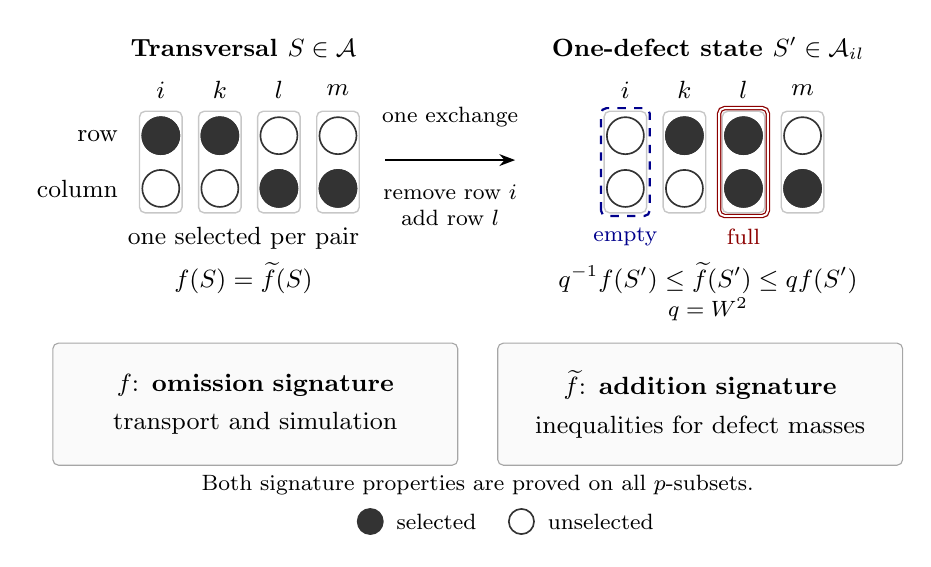
\begin{tikzpicture}[
    x=1cm,y=1cm,
    font=\small,
    element/.style={circle,draw=black!80,line width=.6pt,
      minimum size=4.7mm,inner sep=0pt},
    selected/.style={element,fill=black!80},
    pair/.style={draw=black!22,rounded corners=2pt,line width=.5pt},
    lift/.style={draw=black!35,rounded corners=2pt,
      fill=black!2,align=center,inner sep=7pt,
      text width=4.65cm,minimum height=1.55cm}
  ]
    \node[font=\small\bfseries] at (2.2,2.52) {Transversal $S\in\mathcal A$};
    \node[font=\small\bfseries] at (8.1,2.52) {One-defect state $S'\in\mathcal A_{il}$};

    \foreach \x/\lab in {1.15/i,1.90/k,2.65/l,3.40/m} {
      \draw[pair] (\x-.27,.43) rectangle (\x+.27,1.72);
      \node at (\x,1.99) {$\lab$};
      \node[element] at (\x,1.41) {};
      \node[element] at (\x,.74) {};
    }
    \node[anchor=east] at (.73,1.41) {row};
    \node[anchor=east] at (.73,.74) {column};
    \foreach \x/\y in {1.15/1.41,1.90/1.41,2.65/.74,3.40/.74}
      \node[selected] at (\x,\y) {};
    \node at (2.2,.11) {one selected per pair};
    \node at (2.2,-.40) {$f(S)=\widetilde f(S)$};

    \foreach \x/\lab in {7.05/i,7.80/k,8.55/l,9.30/m} {
      \draw[pair] (\x-.27,.43) rectangle (\x+.27,1.72);
      \node at (\x,1.99) {$\lab$};
      \node[element] at (\x,1.41) {};
      \node[element] at (\x,.74) {};
    }
    \foreach \x/\y in {7.80/1.41,8.55/1.41,8.55/.74,9.30/.74}
      \node[selected] at (\x,\y) {};
    \draw[draw=blue!55!black,dashed,rounded corners=2pt,line width=.8pt]
      (6.74,.39) rectangle (7.36,1.76);
    \draw[draw=red!55!black,double,double distance=.7pt,
      rounded corners=2pt,line width=.45pt]
      (8.24,.39) rectangle (8.86,1.76);
    \node[font=\footnotesize,text=blue!55!black] at (7.05,.12) {empty};
    \node[font=\footnotesize,text=red!55!black] at (8.55,.12) {full};
    \node at (8.1,-.40) {$q^{-1}f(S')\leq\widetilde f(S')\leq qf(S')$};
    \node[font=\footnotesize] at (8.1,-.80) {$q=W^2$};

    \draw[-{Stealth[length=2mm]},line width=.7pt]
      (4.00,1.10) -- (5.65,1.10);
    \node[font=\footnotesize,align=center] at (4.825,1.65)
      {one exchange};
    \node[font=\footnotesize,align=center] at (4.825,.53)
      {remove row $i$\\add row $l$};

    \node[lift] at (2.35,-2.00)
      {$f$: \textbf{omission signature}\\[3pt]
       transport and simulation};
    \node[lift] at (8.00,-2.00)
      {$\widetilde f$: \textbf{addition signature}\\[3pt]
       inequalities for defect masses};
    \node[font=\footnotesize] at (5.175,-3.02)
      {Both signature properties are proved on all $p$-subsets.};
    \node[selected,minimum size=3.2mm] at (3.81,-3.49) {};
    \node[anchor=west,font=\footnotesize] at (4.02,-3.49) {selected};
    \node[element,minimum size=3.2mm] at (5.73,-3.49) {};
    \node[anchor=west,font=\footnotesize] at (5.94,-3.49) {unselected};
  \end{tikzpicture}
  \caption{The paired state space and the two factorial lifts, illustrated with
  four pairs. The lifts agree on transversals. Their comparison within a factor
  $q$ is used only on transversals and one-defect types. The distinct signature
  properties support the two different parts of the argument shown below the
  states.}
  \label{fig:paired-states}
\end{figure}


\subsection{Defect masses and pair inequalities}

Fix \(j\), put \(C=C(j)\), and suppress the parameter on both lifts.
A partial transversal assignment \(\sigma\) specifies one chosen
element in each of a collection of labeled pairs.
A set respects \(\sigma\) when its intersection with every assigned
pair is precisely that chosen element.
For unassigned distinct pair labels \(i,l\), define
\begin{align*}
 z_\sigma
 &=\sum_{\substack{S\in\mathcal A\\S\text{ respects }\sigma}}f(S)
   =\sum_{\substack{S\in\mathcal A\\S\text{ respects }\sigma}}
       \widetilde f(S),\\
 c_{il}^{\sigma}
 &=\sum_{\substack{S\in\mathcal A_{il}\\
                   S\text{ respects }\sigma}}f(S),
 \qquad
 \widetilde c_{il}^{\sigma}
 =\sum_{\substack{S\in\mathcal A_{il}\\
                  S\text{ respects }\sigma}}\widetilde f(S).
\end{align*}
These masses are positive.
For the empty assignment we write \(c_{il},\widetilde c_{il}\)
without a superscript and have \(z_\varnothing=C\).

\begin{lemma}[Pair inequalities for defect masses]
\label{lem:defect-inequalities}
For every partial assignment \(\sigma\) and distinct unassigned
labels \(i,l\),
\begin{equation}
 4\widetilde c_{il}^{\sigma}\widetilde c_{li}^{\sigma}
 \le z_\sigma^2.
 \label{eq:defect-two-pair}
\end{equation}
For three distinct unassigned labels \(i,l,k\),
\begin{equation}
 \widetilde c_{il}^{\sigma}\widetilde c_{lk}^{\sigma}
 \le z_\sigma\widetilde c_{ik}^{\sigma}.
 \label{eq:defect-three-pair}
\end{equation}
\end{lemma}

\begin{proof}
Fix the inclusions and exclusions specified by \(\sigma\).
For \eqref{eq:defect-two-pair}, sum every other unassigned pair at
occupancy one, leaving only \(i,l\).
By Lemma~\ref{lem:binary-signatures}, the remaining positive
two-element weight has an addition matrix with at most one
positive eigenvalue.
Restrict its quadratic form to vectors constant on each of the two
pairs.
The resulting matrix is
\[
 \begin{pmatrix}
  2\widetilde c_{li}^{\sigma}&z_\sigma\\
  z_\sigma&2\widetilde c_{il}^{\sigma}
 \end{pmatrix}.
\]
The diagonal factor two counts the two orders of the elements in
a full pair; the off-diagonal sums exactly the transversals.
The matrix has positive trace and at most one positive eigenvalue,
so its determinant is nonpositive.
This proves \eqref{eq:defect-two-pair}.

For \eqref{eq:defect-three-pair}, sum every other unassigned pair
at occupancy one, leaving the six elements in \(i,l,k\) and a
positive weight on their three-element subsets.
Form its symmetric cubic tensor, zero on repeated indices.
Contract it along the indicator of the two elements of pair \(k\).
By the full-matrix assertion of
Lemma~\ref{lem:binary-contraction}, the resulting matrix has at
most one positive eigenvalue even while the two contracted indices
are retained.
Restrict its form to vectors constant on each pair, and call the
resulting three-by-three matrix \(N\), indexed by \(i,l,k\).
Its relevant entries are
\begin{equation}
 N_{ll}=2\widetilde c_{il}^{\sigma},
 \qquad
 N_{ik}=2\widetilde c_{lk}^{\sigma},
 \qquad
 N_{il}=z_\sigma,
 \qquad
 N_{lk}=2\widetilde c_{ik}^{\sigma}.
 \label{eq:contracted-defect-entries}
\end{equation}
For example, in \(N_{ik}\) the full pair \(k\) can contribute either
of its elements to the contraction and the other to the matrix
index, explaining the factor two.
All entries of \(N\) are nonnegative, and \(N_{ll}>0\).

By \eqref{eq:signature-projection}, the Schur complement against
the \(l,l\) entry is negative semidefinite.
Its two remaining coordinates \(i,k\) therefore satisfy
\begin{align*}
 N_{ik}
 &\le \frac{N_{il}N_{lk}}{N_{ll}}
 +\sqrt{
   \left(\frac{N_{il}^2}{N_{ll}}-N_{ii}\right)
   \left(\frac{N_{lk}^2}{N_{ll}}-N_{kk}\right)}\\
 &\le \frac{2N_{il}N_{lk}}{N_{ll}}.
\end{align*}
The square-root factors are nonnegative by the same Schur
complement condition.
The second inequality uses \(N_{ii},N_{kk}\ge0\) and the
nonnegativity of the off-diagonal entries.
Substituting \eqref{eq:contracted-defect-entries} gives
\eqref{eq:defect-three-pair}.
\end{proof}

The omission property of $f$ is the input to the one-hole transport
argument in Section~\ref{sec:transport}; it applies even to auxiliary
completions outside the enlarged state space.  The two addition-based
inequalities just proved control the conditional and unconditional
one-defect masses used to bound transversal variance and defect means.
The comparison of the lifts is used only on the actual transversal
and one-defect classes where \eqref{eq:lift-comparison} holds.

The matrices and balanced sums used to prove the signature
properties are analytic devices.
The algorithm will neither form these matrices nor enumerate their
underlying coordinate boxes.

\section{Transport, observable variance, and trace mixing}
\label{sec:transport}

Fix an annealing parameter $j$ and suppose that $p\geq 1$.
Write $f=f_j$, $\widetilde f=\widetilde f_j$, and $C=C(j)$.
We use the paired ground set, transversal class $\mathcal A$, defect
classes $\mathcal A_{il}$, and their conditional masses from
Section~\ref{sec:signatures}. In particular, $f$ is positive on
\emph{all} $p$-subsets of the $2p$ elements, and has the omission
property. The second lift $\widetilde f$ has the addition property.
They agree on transversals and satisfy the comparison
\eqref{eq:lift-comparison}, with $q=W^2$, on the state space
\[
  \mathcal X=\mathcal A\,\cup\!
       \bigcup_{\substack{1\leq i,l\leq p\\i\ne l}}\mathcal A_{il}.
\]
We give signed-flow, observable-variance, and trace arguments for these
two lifts, keeping track of the comparison factors and of the domains
on which they are needed. The flow-energy and trace viewpoints are
classical; see Aldous and Fill~\cite[Sections~2.7.1 and~3.7.1]{AF2002}.
The transport inequality first bounds transversal variance and defect
means; together these control the particular trajectory averages used
by the algorithm. The transversal variance bound also gives mixing
of the transversal trace, whose return-time analysis bounds its cost.

We adapt the paired-transversal transport and observable/trace analysis
for counting common bases of two matroids
in~\cite[Sections~4--6]{OpenAICommonBases2026}.
Here the two required signature properties belong to separate lifts.
Their comparison contributes the factors $q^2$ and $q^3$ in the
transversal-variance and defect-mean bounds below. We give the complete
argument for these weights.

\subsection{The enlarged Metropolis chain}

For each ordered pair $i\ne l$, choose a positive multiplier $w_{il}$,
and put
\[
 \lambda(S)=
 \begin{cases}
   f(S),&S\in\mathcal A,\\
   w_{il}f(S),&S\in\mathcal A_{il}.
 \end{cases}
 \qquad
 \Lambda=\sum_{S\in\mathcal X}\lambda(S),
 \qquad
 \pi(S)=\frac{\lambda(S)}{\Lambda}.
\]
Call the multipliers \emph{good} if
\begin{equation}
 \frac{C}{4c_{il}}\leq w_{il}\leq\frac{4C}{c_{il}}
 \qquad(i\ne l).
 \label{eq:good-multipliers}
\end{equation}
For good multipliers,
\begin{equation}
 \Lambda\leq \bigl(1+4p(p-1)\bigr)C\leq 5p^2C,
 \qquad
 \pi(\mathcal A)\geq\frac{1}{5p^2},
 \qquad
 \pi(\mathcal A_{il})\geq\frac{1}{20p^2}.
 \label{eq:type-mass-bounds}
\end{equation}
Indeed, a defect type has total multiplied mass between $C/4$ and
$4C$, and the transversal mass is $C$. When $p=1$ there are no defect
types; all assertions concerning them are omitted.

The chain holds with probability $1/2$. Otherwise it independently
chooses one uniform element of $S$ and one uniform element of its
complement and proposes to exchange them. A proposal outside
$\mathcal X$ is rejected. A proposal $S'$ in $\mathcal X$ is accepted
with probability
$\min\{1,\lambda(S')/\lambda(S)\}$.
Denote its transition operator by $P$.
Every defect state can reach a transversal by moving one element of
its full pair to its empty pair. Transversals are connected by flips
within individual pairs. Positivity of $\lambda$ therefore makes the
chain irreducible. Its holding probability is at least $1/2$.
For distinct exchange neighbors,
\[
 \pi(S)P(S,S')=
 \frac{\min\{\lambda(S),\lambda(S')\}}{2p^2\Lambda},
\]
so $P$ is reversible with stationary law $\pi$.
For a real function $g$ on $\mathcal X$, define
\begin{align}
 \mathfrak D(g)
   &=\sum_{\{S,S'\}}
       \min\{\lambda(S),\lambda(S')\}
          \bigl(g(S)-g(S')\bigr)^2,
 \notag\\
 \mathcal E(g)
   &=\langle g,(I-P)g\rangle_\pi
     =\frac{\mathfrak D(g)}{2p^2\Lambda}.
 \label{eq:energy}
\end{align}
The sum is over unordered exchange edges in $\mathcal X$.
This convention will be used throughout the section.

\subsection{A transport inequality on one-hole states}

The next lemma uses the omission property of $f$ on its full domain.
Some configurations contributing to its auxiliary masses need not
belong to $\mathcal X$. Its applications will identify the one-hole states and
their conductances with actual states and conductances of the
Metropolis chain.

\begin{lemma}[One-hole transport]
\label{lem:transport}
Fix disjoint sets of included and excluded elements. Let $F$ be the
set of fixed inclusions, and partition the remaining elements into two
singleton slots $P_0,P_1$ and $s$ ordinary slots of two elements each.
Assume $|F|+s+1=p$.
Let $\mathcal X_{\mathrm{sl}}$ consist of the sets that respect the
fixed assignments and select one element from every slot except one
hole slot, from which they select nothing.
Give a state with hole slot $i$ weight $W_i f(S)$, where every $W_i$ is
positive. For a real function $g$ on $\mathcal X_{\mathrm{sl}}$, let
$D_{\mathrm{sl}}(g)$ be the unordered-edge energy on its single-exchange
graph, with conductance equal to the minimum of the two endpoint weights.

Let $s_0,s_1$ be the unmultiplied $f$-masses of the states with hole
$P_0,P_1$, and let $\bar g_0,\bar g_1$ be their respective $f$-weighted
means. For each ordinary slot $t$, let $v_t$ be the unmultiplied mass
of sets that omit both singleton slots, select both elements of $t$,
and select one element from every other ordinary slot, while
respecting the fixed assignments. Then
\begin{equation}
 (\bar g_0-\bar g_1)^2
 \leq
 \left(
   \frac{1}{s_0W_{P_0}}+\frac{1}{s_1W_{P_1}}
   +\frac{2}{s_0s_1}\sum_t\frac{v_t}{W_t}
 \right)D_{\mathrm{sl}}(g).
 \label{eq:slot-transport}
\end{equation}
The notation $W_i$ here denotes slot multipliers, independently of the
capacity threshold $W$.
\end{lemma}

\begin{proof}
We seek a signed edge current whose divergence is $f(S)/s_0$ at
states with hole $P_0$, $-f(S)/s_1$ at states with hole $P_1$, and zero
at all ordinary-hole states. Orient each edge once, write $I_{SS'}$
for its signed current, and write $c_{SS'}$ for its conductance.
Such a current satisfies, by summation by parts and Cauchy--Schwarz,
\begin{equation}
 \begin{split}
  (\bar g_0-\bar g_1)^2
   &=\left(\sum_{\{S,S'\}}
                 I_{SS'}\bigl(g(S)-g(S')\bigr)\right)^2\\
   &\leq
      \left(\sum_{\{S,S'\}}\frac{I_{SS'}^2}{c_{SS'}}\right)
      D_{\mathrm{sl}}(g).
 \end{split}
 \label{eq:transport-flow-criterion}
\end{equation}
It therefore suffices to bound its flow energy by the coefficient in
\eqref{eq:slot-transport}.

The local routing step explains the energy quantity we will use.
A complete display $R$ contains the two singleton elements and one
chosen element from every ordinary slot. Its one-hole sets
$S_i=F\cup(R\setminus\{i\})$, $i\in R$, form a clique of exchange
edges. For an element $i$, write $W_i$ for its slot's multiplier.
Put $m_i=f(S_i)$. For any coefficients $h_i$ with
$\sum_i m_i h_i=0$, regard $m_i h_i$ as the prescribed signed
divergence at $S_i$. Choose a hub $h_*$ maximizing $W_i m_i$, and
send current $m_i h_i$ from each nonhub $S_i$ to the hub. Balance gives
the prescribed divergence at the hub as well. Each used edge has
conductance $W_i m_i$ at its nonhub endpoint, so this routing has
energy at most
\[
 \sum_{i\ne h_*}\frac{(m_i h_i)^2}{W_i m_i}
 \leq\sum_{i\in R}\frac{m_i h_i^2}{W_i}.
\]
We now assign these balanced demands recursively. Their sum over
complete displays will have the required source and sink divergences;
the recursion will also bound the sum of their routing energies.

Fix an order of the ordinary slots. Initially display the two
singleton elements. Expose ordinary slots in that order, branching
into two children according to which element of the next slot is
added to the display.
At a node write $R$ for its displayed elements, excluding $F$.
For $i\in R$, let $m_i$ be the sum of $f$ over sets that contain
$F\cup(R\setminus\{i\})$, omit the nondisplayed mates in already
processed slots, and have single occupancy in every unprocessed
ordinary slot. These sets all have size $p$, and $m_i>0$.
At a complete display this definition reduces to $m_i=f(S_i)$.
Maintain coefficients $h_i$, interpreted as demand per unit
unmultiplied weight, satisfying
\begin{equation}
  \sum_{i\in R}m_i h_i=0.
  \label{eq:transport-balance}
\end{equation}
At the root their values are $1/s_0$ and $-1/s_1$ at the elements of
$P_0$ and $P_1$, respectively. Assign the node the potential
\[
  \Psi(R,h)=\sum_{i\in R}\frac{m_i h_i^2}{W_i}.
\]
At a leaf this potential bounds the routing energy just computed. Each $W_i$
is fixed by its slot throughout the recursion. These multipliers
enter the energy bound and the eventual hub choice, but not the
recursive coefficients or prescribed divergences.

Suppose the next slot $t$ has elements $a,b$.
For an old hole $i\in R$, let $m_i^a,m_i^b$ be its masses in the two
children. Then $m_i^a+m_i^b=m_i$.
The mass of the newly introduced hole, at $a$ in the first child and
at $b$ in the second, is the same positive number $u$: in either case
the entire slot $t$ is empty.
Put $X=\sum_{i\in R}h_i m_i^a$.
Retain every old coefficient unchanged, and give the new hole
coefficient $-X/u$ in the $a$ child and $X/u$ in the $b$ child.
Equation~\eqref{eq:transport-balance} holds in both children because
$\sum_i h_i m_i^b=-X$.
The sum of their potentials exceeds the parent potential by exactly
\begin{equation}
  \frac{2X^2}{uW_t}.
  \label{eq:transport-increment}
\end{equation}

We bound these increments using the omission signature. At any node,
and for any unprocessed ordinary slot $t$, define a symmetric matrix
$V_t(R)$ on the displayed elements, with zero diagonal. For distinct
$i,k\in R$, its entry is the sum of $f$ over configurations with holes
at $i,k$ in the display, double occupancy in slot $t$, and single
occupancy in every other unprocessed slot. Fixed inclusions,
exclusions, and previously excluded mates remain in force.
All these configurations have size $p$.

When $t=\{a,b\}$ is the next slot, $V_t(R)$ is the old block of
\[
 N=\begin{pmatrix}
     V_t(R)&(m_i^b)_{i\in R}&(m_i^a)_{i\in R}\\
     (m_i^b)_{i\in R}^{\mathsf T}&0&u\\
     (m_i^a)_{i\in R}^{\mathsf T}&u&0
   \end{pmatrix}.
\]
This form has at most one positive eigenvalue. To see the precise
application, fix the context and exclude the nondisplayed mates of
processed slots. Sum all unprocessed ordinary slots other than $t$
at occupancy one. On the remaining ground set $R\cup\{a,b\}$ the
resulting degree is $|R|$, so $N$ is its two-omission matrix.
Lemmas~\ref{lem:binary-signatures} and
\ref{lem:binary-contraction} give the asserted signature.
In particular, this argument uses the full-domain weight $f$ even
when an entry of $V_t(R)$ describes multiple empty and full original
pairs. No comparison with $\widetilde f$ is made here.

Extend $h$ by zero at $a,b$ and put $d_{ab}=e_a-e_b$.
The vector $e_a+e_b$ has square $2u>0$ under $N$.
Both $h$ and $d_{ab}$ are orthogonal to it in this form, since
\eqref{eq:transport-balance} holds and the two new diagonal entries
are zero. A symmetric form with at most one positive eigenvalue is
nonpositive on the form-orthogonal complement of a positive-square
vector: another positive-square vector in that complement would span
a positive definite plane with the first vector. On the complement,
Cauchy--Schwarz for the negative of the form applies. Here
\[
 h^{\mathsf T}N d_{ab}=-2X,
 \qquad d_{ab}^{\mathsf T}N d_{ab}=-2u,
 \qquad h^{\mathsf T}Nh=h^{\mathsf T}V_t(R)h.
\]
Consequently
\begin{equation}
   \frac{2X^2}{u}\leq -h^{\mathsf T}V_t(R)h.
   \label{eq:transport-schur}
\end{equation}

Fix now a slot $t$ to be processed at a later level.
When a preceding slot is split, the sum of the two child quantities
$h^{\mathsf T}V_t(R)h$ equals the parent quantity.
The old entries split additively. A cross entry involving the new
hole represents a configuration in which the split slot is empty,
so it is identical in the two children. Its contributions cancel
because the new coefficients are opposite and all old coefficients
are retained. There is no new diagonal contribution.
Iterating this identity shows that, immediately before processing
$t$, the sum of these quadratic quantities over the whole level
is their value at the root. The root matrix has off-diagonal entry
$v_t$ and zero diagonal, so that value is
$-2v_t/(s_0s_1)$.
By \eqref{eq:transport-increment} and
\eqref{eq:transport-schur}, the total potential increase at the level
of slot $t$ is at most $2v_t/(s_0s_1W_t)$.
The root potential is
$1/(s_0W_{P_0})+1/(s_1W_{P_1})$.
Thus the sum of all leaf potentials is bounded by the parenthetical
coefficient in \eqref{eq:slot-transport}.

Route the prescribed demands at every leaf by the clique construction
above. Its energy is at most $\Psi(R,h)$.
Different leaves cannot use the same edge: the union of two distinct
endpoints of a leaf edge is exactly $F\cup R$, and so determines the
entire display and its unique sequence of choices. Hence the assembled
flow has energy at most the sum of the leaf potentials.

It remains to identify the divergence after summing the leaf flows.
A state with a singleton hole has one leaf representation; its
divergence is $f(S)/s_0$ or $-f(S)/s_1$.
A state $S$ with an ordinary hole at slot $t$ has exactly two
representations, obtained by adjoining either element of $t$ to
$S\setminus F$. Every other displayed ordinary choice is fixed by
$S$. The two histories agree before processing $t$, so the same
$X,u$ create opposite coefficients there. Those coefficients remain
unchanged at every later branch, regardless of the later masses and
new coefficients. At the leaves both masses are exactly $f(S)$,
and their divergences cancel. This reasoning also applies if the
state is a hub in either leaf, since its net divergence is still
$m_i h_i$.
The assembled flow therefore has the required divergence, and
\eqref{eq:transport-flow-criterion} together with the leaf-potential
bound proves \eqref{eq:slot-transport}. If $s=0$, the root is already
a complete display and the same clique argument applies directly.
\end{proof}

\subsection{Variance on transversals}

Assume henceforth that the multipliers are good, and write
\[
  \mu(S)=\frac{f(S)}{C}\quad(S\in\mathcal A),
  \qquad C_{\mathrm p}=p(1+8pq^2).
\]
The variance under $\mu$ of a function on $\mathcal X$ refers to its
restriction to $\mathcal A$.

\begin{proposition}
\label{prop:transversal-variance}
Suppose the multipliers satisfy~\eqref{eq:good-multipliers}.
For every real function $g$ on $\mathcal X$,
\begin{equation}
    C\Var_\mu(g)\leq C_{\mathrm p}\mathfrak D(g).
    \label{eq:transversal-variance}
\end{equation}
\end{proposition}

\begin{proof}
We decompose the transversal variance along a tree of partial
assignments, choosing the next pair as a function of the current
assignment. Let $\sigma$ fix some pairs to specified single choices.
For distinct unassigned labels define
\[
 a_{il}=
  \frac{\widetilde c_{il}^{\sigma}}{z_\sigma}
  \frac{\widetilde c_{li}}{C}.
\]
Lemma~\ref{lem:defect-inequalities} gives
\begin{equation}
 a_{il}a_{li}\leq\frac1{16},
 \qquad
 a_{il}a_{lk}\leq a_{ik}
 \quad\text{for distinct }i,l,k.
 \label{eq:sink-products}
\end{equation}
For the second inequality, use the conditional defect inequality
on the first factors and the unconditioned inequality with indices
$k,l,i$ on the second factors.
Form a directed graph with arc $i\to l$ when $a_{il}>1$.
It has no directed two-cycle. A shortest longer directed cycle could
be shortened using the second inequality in
\eqref{eq:sink-products}, also a contradiction.
Thus this graph has a sink $k$, for which $a_{kt}\leq1$ at every other
unassigned label $t$. If only one label remains, choose it as $k$.

Branch on the two choices in pair $k$.
Apply Lemma~\ref{lem:transport} with the two elements of $k$ as
singleton slots, both of multiplier one, and with the other
unassigned pairs as ordinary slots. Keep $\sigma$ fixed.
A singleton-hole state is a transversal respecting $\sigma$; an
ordinary-hole state at $t$ has type $tk$ and multiplier $W_t=w_{tk}$.
The auxiliary doubled-slot mass is exactly $v_t=c_{kt}^\sigma$.
Thus every one-hole state in this application belongs to
$\mathcal X$ with precisely its weight $\lambda$.
The good-multiplier bound, followed by two uses of
\eqref{eq:lift-comparison}, gives
\begin{align}
 \frac{v_t}{W_t}
  =\frac{c_{kt}^\sigma}{w_{tk}}
  &\leq\frac{4c_{kt}^\sigma c_{tk}}{C}
   \leq\frac{4q^2\widetilde c_{kt}^\sigma
                        \widetilde c_{tk}}{C}
 \notag\\
  &=4q^2z_\sigma a_{kt}\leq4q^2z_\sigma.
 \label{eq:sink-comparison}
\end{align}
These comparisons involve only actual defect types.

Let $s_0,s_1$ and $\bar g_0,\bar g_1$ be the masses and means of the
two transversal children, so $s_0+s_1=z_\sigma$.
Their unnormalized between-means variance contribution is
\[
   \frac{s_0s_1}{z_\sigma}(\bar g_0-\bar g_1)^2.
\]
Let $\mathfrak D_\sigma(g)$ be the sum in
\eqref{eq:energy} restricted to edges whose two endpoints respect
$\sigma$. The slot energy in this application is a subgraph energy,
so it is at most $\mathfrak D_\sigma(g)$.
Multiplying \eqref{eq:slot-transport} by $s_0s_1/z_\sigma$ and using
\eqref{eq:sink-comparison} yields
\begin{equation}
 \frac{s_0s_1}{z_\sigma}(\bar g_0-\bar g_1)^2
 \leq (1+8pq^2)\mathfrak D_\sigma(g).
 \label{eq:conditional-variance-charge}
\end{equation}
The first two terms in the transport coefficient contribute exactly
$(s_0+s_1)/z_\sigma=1$; the ordinary slots contribute at most
$8pq^2$.

Iterate this branching until every pair is fixed. The conditional
variance identity decomposes $C\Var_\mu(g)$ as the sum of the
between-means contributions over the internal nodes.
At any depth, two distinct nodes disagree on the choice of the pair
fixed at their first divergence. Their restricted state sets are
disjoint, even if subsequent pairs were chosen in different orders.
Consequently their internal edge sets are disjoint and
\[
  \sum_{\sigma\text{ at a fixed depth}}\mathfrak D_\sigma(g)
  \leq\mathfrak D(g).
\]
An edge crossing a fixed-pair choice is internal to neither of the
two resulting restrictions; it does not create a duplicate charge.
There are $p$ possible branching depths. Summing
\eqref{eq:conditional-variance-charge} proves
\eqref{eq:transversal-variance}.
The conditioning tree and sink choices are used only in this proof.
\end{proof}

\subsection{Defect means and observable variance}

Set
\[
  C_{\mathrm d}=8+32pq^3.
\]
For $i\ne l$, let
$\bar g_{il}=c_{il}^{-1}\sum_{S\in\mathcal A_{il}}f(S)g(S)$.

\begin{lemma}
\label{lem:defect-mean}
Suppose the multipliers satisfy~\eqref{eq:good-multipliers}, and let
$g$ be a real function on $\mathcal X$.
For each defect type $il$ there is a conditional transversal mean
$\bar g'$ such that
\begin{equation}
 (\bar g_{il}-\bar g')^2
       \leq \frac{C_{\mathrm d}}{C}\mathfrak D(g),
 \qquad
 (\bar g'-\mathbb E_\mu g)^2\leq4\Var_\mu(g).
 \label{eq:defect-mean-bounds}
\end{equation}
\end{lemma}

\begin{proof}
Of the four possible joint choices in pairs $i,l$, choose one whose
transversal mass is at least $C/4$.
Denote the selected elements by $a_i,a_l$ and their mates by
$b_i',b_l'$.
In Lemma~\ref{lem:transport}, fix $a_l$ included and $b_i'$ excluded,
and take $P_0=\{a_i\}$, $P_1=\{b_l'\}$. All other pairs are ordinary
slots. A hole at $P_0$ gives the entire defect type $il$, whereas a
hole at $P_1$ gives the selected conditional transversal class.
Thus
\[
 s_0=c_{il},\quad W_{P_0}=w_{il},\qquad
 s_1\geq C/4,\quad W_{P_1}=1.
\]
An ordinary hole at $t$ has type $tl$, restricted to the choice $a_i$
in pair $i$, and has multiplier $W_t=w_{tl}$.
A doubled ordinary slot with both singleton slots empty is a subset
of type $it$, so $v_t\leq c_{it}$.
All one-hole states and their exchange edges are therefore genuine
states and edges of the chain, with the same endpoint weights.
Their energy is at most $\mathfrak D(g)$.

The lift comparison and Lemma~\ref{lem:defect-inequalities} give,
for each ordinary slot $t$,
\begin{equation}
 c_{it}c_{tl}
 \leq q^2\widetilde c_{it}\widetilde c_{tl}
 \leq q^2C\widetilde c_{il}
 \leq q^3C c_{il}.
 \label{eq:defect-comparison}
\end{equation}
The first two terms in the coefficient of
\eqref{eq:slot-transport} are at most $4/C+4/C$.
For its last term, \eqref{eq:good-multipliers} and
\eqref{eq:defect-comparison} give
\[
 \frac{2}{s_0s_1}\sum_t\frac{v_t}{W_t}
 \leq\frac{8}{c_{il}s_1C}\sum_t c_{it}c_{tl}
 \leq\frac{8pq^3}{s_1}
 \leq\frac{32pq^3}{C}.
\]
This proves the first inequality of
\eqref{eq:defect-mean-bounds} with $\bar g'$ the selected conditional
mean. The conditioning event has $\mu$-probability at least $1/4$;
conditional Cauchy--Schwarz gives
\[
 (\bar g'-\mathbb E_\mu g)^2
 \leq \mathbb E_\mu\bigl[(g-\mathbb E_\mu g)^2
                        \mid\text{selected choices}\bigr]
 \leq4\Var_\mu(g),
\]
which proves the second inequality.
\end{proof}

Define $\mathcal Q$ on real functions on $\mathcal X$ by retaining
all values on $\mathcal A$ and replacing the values on each defect
type by their mean within that type. Since its multiplier is
constant, the conditional $\pi$-mean on $\mathcal A_{il}$ is
$\bar g_{il}$. Hence $\mathcal Q$ is the orthogonal projection in
$L^2(\pi)$ associated with the partition into individual transversal
states and entire defect types. Its range consists of functions that
are arbitrary on $\mathcal A$ and constant within each defect type.
This includes type indicators and every function supported on
$\mathcal A$, the two kinds of observables used in
Section~\ref{sec:algorithm}. It preserves constants and means.

Chen, Vigoda, and Yang use a restricted variance bound for hole-pattern
frequencies in permanent approximation~\cite[Theorem~5 and
Lemma~12]{CVY2026}. Their partition pools the perfect matchings;
here each transversal is retained separately, while each defect type
is averaged. The inequality below controls this projection without
requiring a bound on all fluctuations within a defect type.
Put
\begin{equation}
  K_{\mathrm{obs}}=10p^4(9C_{\mathrm p}+2C_{\mathrm d}).
  \label{eq:observable-constant}
\end{equation}

\begin{proposition}[Observable variance]
\label{prop:observable-variance}
Suppose the multipliers satisfy~\eqref{eq:good-multipliers}.
For every real $g$ on $\mathcal X$,
\begin{equation}
 \Var_\pi(\mathcal Qg)
 \leq(9C_{\mathrm p}+2C_{\mathrm d})\frac{\mathfrak D(g)}{C}
 \leq K_{\mathrm{obs}}\mathcal E(g).
 \label{eq:observable-variance}
\end{equation}
\end{proposition}

\begin{proof}
Let $m=\mathbb E_\mu g$.
Lemma~\ref{lem:defect-mean} and $(a+b)^2\leq2a^2+2b^2$ give
\[
  (\bar g_{il}-m)^2
  \leq\frac{2C_{\mathrm d}}{C}\mathfrak D(g)
       +8\Var_\mu(g).
\]
Variance is no larger than squared deviation about any fixed
constant. Therefore
\begin{align*}
 \Var_\pi(\mathcal Qg)
 &\leq\mathbb E_\pi[(\mathcal Qg-m)^2]\\
 &=\pi(\mathcal A)\Var_\mu(g)
       +\sum_{i\ne l}\pi(\mathcal A_{il})(\bar g_{il}-m)^2\\
 &\leq9\Var_\mu(g)+\frac{2C_{\mathrm d}}{C}\mathfrak D(g)\\
 &\leq(9C_{\mathrm p}+2C_{\mathrm d})\frac{\mathfrak D(g)}{C},
\end{align*}
using Proposition~\ref{prop:transversal-variance} in the last step.
Finally, \eqref{eq:energy} and \eqref{eq:type-mass-bounds} give
$\mathfrak D(g)/C\leq10p^4\mathcal E(g)$.
When $p=1$ the defect sum is empty and $\mathcal Q=I$; the same
inequalities apply.
\end{proof}

\subsection{Trajectory averages of the controlled observables}

The covariance-sum viewpoint is classical; see
Aldous and Fill~\cite[Section~2.3]{AF2002}. Here we derive the needed
finite-time bound from the restricted observable inequality.

\begin{lemma}[Time averages from a dominated initial law]
\label{lem:time-average}
Suppose the multipliers satisfy~\eqref{eq:good-multipliers}.
Let $G$ be a real function on $\mathcal X$ with $\mathcal QG=G$.
Suppose $S_0$ has law $\nu$ satisfying $\nu(S)\leq U\pi(S)$ for
every state. For $N\geq1$ consecutive observations of the chain,
\begin{equation}
 \mathbb E_\nu\left[
    \left(\frac1N\sum_{t=0}^{N-1}G(S_t)-\mathbb E_\pi G\right)^2
                  \right]
 \leq\frac{2UK_{\mathrm{obs}}}{N}\Var_\pi(G).
 \label{eq:time-average-bound}
\end{equation}
\end{lemma}

\begin{proof}
Write $G_c=G-\mathbb E_\pi G$ and $v=\Var_\pi(G)$.
Because $\mathcal Q$ is an orthogonal projection fixing constants,
for every $g$,
\begin{align*}
 |\langle G_c,g\rangle_\pi|^2
 &=|\langle G_c,\mathcal Qg-\mathbb E_\pi g\rangle_\pi|^2\\
 &\leq v\Var_\pi(\mathcal Qg)
 \leq K_{\mathrm{obs}}v\mathcal E(g).
\end{align*}
On the mean-zero subspace, $I-P$ is positive definite and invertible:
reversibility makes $P$ self-adjoint, and finite irreducibility makes
its eigenvalue one simple. Take
$g=(I-P)^{-1}G_c$ on this subspace and put
\[
 a=\langle G_c,(I-P)^{-1}G_c\rangle_\pi=\mathcal E(g)\geq0.
\]
The previous inequality gives $a^2\leq K_{\mathrm{obs}}va$, and hence
$a\leq K_{\mathrm{obs}}v$, also when $a=0$.

Laziness puts the spectrum of $P$ in $[0,1]$: the operator $2P-I$ is
itself a reversible stochastic contraction. Thus the stationary
covariances
$c_t=\langle G_c,P^tG_c\rangle_\pi$ are nonnegative, and finite
spectral decomposition on the mean-zero subspace gives
\[
  \sum_{t=0}^{\infty}c_t
  =\langle G_c,(I-P)^{-1}G_c\rangle_\pi=a.
\]
For a stationary trajectory the mean squared error of the average is
\[
 \frac{Nv+2\sum_{t=1}^{N-1}(N-t)c_t}{N^2}
 \leq\frac{2a}{N}
 \leq\frac{2K_{\mathrm{obs}}v}{N}.
\]
Finally, the law of an entire trajectory started from $\nu$ is
bounded by $U$ times the corresponding stationary trajectory law:
only the initial factor changes in the product of transition
probabilities. Applying this domination to the nonnegative squared
error proves \eqref{eq:time-average-bound}.
\end{proof}

\subsection{The transversal trace and its return cost}

Starting from $x\in\mathcal A$, let
\[
  T_{\mathcal A}^+=\inf\{t\geq1:S_t\in\mathcal A\},
  \qquad
  P_{\mathrm{tr}}(x,y)
     =\mathbb P_x(S_{T_{\mathcal A}^+}=y).
\]
The trace makes one transition for each strictly positive return to
$\mathcal A$; consecutive visits and original holding steps count
as returns.
The mean return identity used below is the finite-state form of
Kac's formula~\cite[Corollary~2.24]{AF2002}.

\begin{lemma}[Trace mixing and return cost]
\label{lem:trace}
Suppose the multipliers satisfy~\eqref{eq:good-multipliers}.
The trace kernel $P_{\mathrm{tr}}$ is irreducible, reversible with
stationary law $\mu$, and has holding probability at least $1/2$.
Its inverse spectral gap is at most
$2p^2C_{\mathrm p}\leq K_{\mathrm{obs}}$.
In particular, with
$\mu_{\min}=\min_{x\in\mathcal A}\mu(x)>0$, for every integer $s\geq0$,
\begin{equation}
 \left|\frac{P_{\mathrm{tr}}^s(x,y)}{\mu(y)}-1\right|
 \leq\mu_{\min}^{-1}\exp(-s/K_{\mathrm{obs}})
 \qquad(x,y\in\mathcal A).
 \label{eq:trace-relative-mixing}
\end{equation}
If the initial trace law satisfies $\nu\leq U\mu$ pointwise, then
\begin{equation}
  \mathbb E_\nu T_{\mathcal A}^+
       \leq\frac{U}{\pi(\mathcal A)}.
  \label{eq:trace-return-cost}
\end{equation}
Furthermore, at every deterministic trace-step index the law remains
bounded by $U\mu$. The expected total number of underlying
transitions for $s$ trace steps is at most $sU/\pi(\mathcal A)$.
\end{lemma}

\begin{proof}
Finite irreducibility ensures finite expected hitting and return
times to $\mathcal A$. Explicitly, from each state choose a finite
positive-probability path to $\mathcal A$. Finiteness of the state
space gives a common bound on path length and a positive lower
bound on these path probabilities. The Markov property then gives
a geometric bound in blocks on the hitting-time tail. Applying this
after the first transition also bounds the strictly positive return
time. These qualitative bounds justify the harmonic extensions and
occupation sums below; no polynomial estimate is assumed at this
point.

For a function $h$ on $\mathcal A$, let $\widehat h$ be its harmonic
extension
\[
 \widehat h(x)=\mathbb E_x h(S_{T_{\mathcal A}}),
 \qquad T_{\mathcal A}=\inf\{t\geq0:S_t\in\mathcal A\}.
\]
Then $\widehat h=h$ on $\mathcal A$, $(I-P)\widehat h=0$ off
$\mathcal A$, and $(I-P)\widehat h=(I-P_{\mathrm{tr}})h$ on
$\mathcal A$ by conditioning on the first transition. For harmonic
extensions $\widehat h,\widehat k$ of $h,k$, it follows that
\begin{equation}
 \langle \widehat h,(I-P)\widehat k\rangle_\pi
   =\frac{C}{\Lambda}
        \langle h,(I-P_{\mathrm{tr}})k\rangle_\mu.
 \label{eq:trace-bilinear-identity}
\end{equation}
Symmetry of the left side proves reversibility of the stochastic
kernel $P_{\mathrm{tr}}$ with respect to $\mu$, and thus stationarity.
Tracing positive-probability paths of $P$ proves irreducibility.
Also $P_{\mathrm{tr}}(x,x)\geq P(x,x)\geq1/2$.

Let
$\mathcal E_{\mathrm{tr}}(h)
 =\langle h,(I-P_{\mathrm{tr}})h\rangle_\mu$.
Taking $k=h$ in \eqref{eq:trace-bilinear-identity} gives the exact
normalization
\[
  \mathfrak D(\widehat h)
    =2p^2\Lambda\mathcal E(\widehat h)
    =2p^2C\mathcal E_{\mathrm{tr}}(h).
\]
Proposition~\ref{prop:transversal-variance} therefore implies
\[
  \Var_\mu(h)\leq2p^2C_{\mathrm p}\mathcal E_{\mathrm{tr}}(h).
\]
This is the stated inverse-gap bound. The inequality
$2p^2C_{\mathrm p}\leq K_{\mathrm{obs}}$ follows immediately from
\eqref{eq:observable-constant} and $p\geq1$.

For the pointwise estimate put
$e_x(z)=\mathbf 1_{\{x\}}(z)/\mu(x)-1$.
Reversibility and spectral contraction on mean-zero functions give
\begin{align*}
 \left|\frac{P_{\mathrm{tr}}^s(x,y)}{\mu(y)}-1\right|
  &=|\langle e_x,P_{\mathrm{tr}}^s e_y\rangle_\mu|\\
  &\leq\exp(-s/K_{\mathrm{obs}})
        \sqrt{\bigl(\mu(x)^{-1}-1\bigr)
                    \bigl(\mu(y)^{-1}-1\bigr)}\\
  &\leq\mu_{\min}^{-1}\exp(-s/K_{\mathrm{obs}}),
\end{align*}
which proves \eqref{eq:trace-relative-mixing}.

To compute the mean return cost, start the underlying chain with law
$\mu$ on $\mathcal A$ and define the finite occupation measure
\[
  m(z)=\mathbb E_\mu
       \sum_{t=0}^{T_{\mathcal A}^+-1}\mathbf 1_{\{S_t=z\}}.
\]
Shifting the sum by one transition removes the initial law and adds
the return law. Both are $\mu$, since the trace is stationary.
Thus $mP=m$. Uniqueness of the stationary probability measure for
the finite irreducible chain implies $m=c\pi$ for some positive
constant $c$. Before the return, the only visit to $\mathcal A$ is at
time zero, so $m$ restricted to $\mathcal A$ is exactly $\mu$.
Consequently $c\pi(\mathcal A)=1$ and
\[
  \mathbb E_\mu T_{\mathcal A}^+
   =\sum_zm(z)=\frac{1}{\pi(\mathcal A)}.
\]
Pointwise domination of the starting law proves
\eqref{eq:trace-return-cost}.
Since $\mu$ is stationary for the trace,
$\nu P_{\mathrm{tr}}^r\leq U\mu$ for every deterministic integer
$r\geq0$. Applying \eqref{eq:trace-return-cost} to each of these
laws and using the Markov property at return times bounds the
expected sum of $s$ excursion lengths by $sU/\pi(\mathcal A)$.
This last bound is unconditional at the deterministic trace indices;
it does not assert domination after conditioning on an arbitrary
past event or on meeting a running-time cap.

When $p=1$, every state is a transversal, $P_{\mathrm{tr}}=P$, and
every return costs exactly one underlying transition. The stated
bounds include this case.
\end{proof}

The flows, auxiliary matrices, and adaptive conditioning trees in
this section certify the estimates but are not constructed by the
algorithm. Section~\ref{sec:algorithm} uses the directly simulated
Metropolis chain, the controlled observables, and capped trace
restarts, together with the bounded weight evaluator from
Proposition~\ref{prop:weight-oracle}.

\section{A bounded approximation procedure for the weights}
\label{sec:evaluation}

The free large coordinates in \eqref{eq:hj} cannot be enumerated in
polynomial time.  We instead partition their ranges into polynomially
many intervals per coordinate and sample the resulting product grid.
Scaled free coordinates, softened constraints, and grid walks appear
in the dense-table methods of Dyer, Kannan, and Mount~\cite{DKM1997};
Morris~\cite{Morris2002} further developed the associated geometric
rounding approach. The weighted bin construction below includes its
geometric estimate, population correction, and finite-bit
implementation in full.

\begin{samepage}
\begin{proposition}[Weight evaluation]
\label{prop:weight-oracle}
Fix a box-valid small-count profile $(x,y)$ with total $p$, an integer
$0\le j\le H$, and rational parameters
$0<\xi_{\mathrm{in}},\theta<1/4$.  There is a randomized procedure
returning a positive rational $\widehat h$ such that
\[
 \mathbb P\left[
  (1-\xi_{\mathrm{in}})h_j(x,y)\le\widehat h
       \le(1+\xi_{\mathrm{in}})h_j(x,y)
 \right]\ge1-\theta.
\]
On every execution its bit cost is bounded by a fixed polynomial in
$L,\epsilon^{-1},\xi_{\mathrm{in}}^{-1},\theta^{-1}$ and the encoding
lengths of the parameters.  If
$M_f=\prod_{s\ \mathrm{free}}(b_s+1)$, every returned value satisfies
\begin{equation}
 \frac{M_f2^{-j}}{16}\le\widehat h\le8M_f.
 \label{eq:oracle-unconditional-range}
\end{equation}
In particular, positivity and the representation-length bound do not
depend on the statistical success event.
\end{proposition}
\end{samepage}

\subsection{Bins and a comparable continuous density}

Throughout the construction, fix $(x,y)$.  Let $e$ be the number of free
cells.  We first describe the positive-dimensional case; the case $e=0$
is addressed below.  On $[0,B]^e$, write $D(v)$ for the penalty of the
free values $z_s=(b_s+1)v_s/B$.  Lemma~\ref{lem:forest} gives
\begin{equation}
 0\le D(v)\le H,
 \qquad
 |D(v)-D(w)|\le\frac{2Ad^2}{B}\|v-w\|_\infty
                   =\frac18\|v-w\|_\infty.
 \label{eq:scaled-penalty-bounds}
\end{equation}
The function $D$ is convex.

Let $\mathcal V=\{0,\ldots,B-1\}^e$ be the bin indices.  Assign an
integer free vector $z$ to the bin whose coordinates are
$\lfloor Bz_s/(b_s+1)\rfloor$.  Denote the resulting Cartesian product
of integer intervals by $I_v$.  In a coordinate with $N=b_s+1$, the
interval for bin index $v_s$ is
\[
 \left\{\left\lceil\frac{Nv_s}{B}\right\rceil,
 \ldots,
 \left\lceil\frac{N(v_s+1)}{B}\right\rceil-1\right\}.
\]
Its cardinality differs from $N/B$ by at most one.  Since a free cell
is large, $N\ge W=100dB$, so every interval is nonempty.  Define
\[
 \alpha_v=\frac{B^e|I_v|}{M_f}.
\]
Each coordinate contributes a factor in
$[1-1/(100d),1+1/(100d)]$.  There are at most $d$ coordinates, and hence
\begin{equation}
 \frac12\le\alpha_v\le2.
 \label{eq:bin-populations}
\end{equation}
The intervals and $\alpha_v$ are computed by integer arithmetic.

For an integer $0\le a\le j$, put
\[
 V_a(v)=2^{-\lfloor aD(v)/H\rfloor},
 \qquad
 \varrho_a(w)=2^{-aD(w)/H}\quad(w\in[0,B]^e).
\]
The density $\varrho_a$ is positive and log-concave.  Its base-two
logarithm has sup-norm Lipschitz constant at most $1/8$, and therefore
also at most one.  Combining this weaker bound with the floor gives,
on the unit bin with lower corner $v$,
\begin{equation}
 \frac{V_a(v)}4\le\varrho_a(w)\le2V_a(v).
 \label{eq:bin-density-comparison}
\end{equation}
The same inequalities hold at boundary points by continuity.

\subsection{The estimator and its population correction}

For $0\le a\le j$, define the bin partition function and law
\[
 S_a=\sum_{v\in\mathcal V}V_a(v),\qquad
 \pi_a(v)=\frac{V_a(v)}{S_a}.
\]
The dyadic weights $V_a$ will permit exact finite-bit Metropolis
acceptance. Their normalizing constants can be estimated through
adjacent ratios. For $0\le a<j$, the observable
\[
 R_a(v)=\frac{V_{a+1}(v)}{V_a(v)}
\]
has expectation $S_{a+1}/S_a$ under $\pi_a$.  Its values are $1/2$ or
one: $0\le D/H\le1$ makes the increment of the floor exponent zero
or one.

For the final correction, draw $v$ from $\pi_j$, then a uniform integer
point $z\in I_v$, and let $s$ be its cube coordinates
$s_u=Bz_u/(b_u+1)$.  Use
\begin{equation}
 T(v,z)=\alpha_v\frac{2^{-jD(s)/H}}{V_j(v)}.
 \label{eq:oracle-correction}
\end{equation}
Equations~\eqref{eq:bin-populations} and
\eqref{eq:bin-density-comparison} show $1/8\le T\le4$.
The factor $\alpha_v$ corrects for the number of integer points in
the selected bin. The correction therefore has exact expectation
\[
 \mathbb E T
 =\frac{1}{S_j}\sum_v\frac{\alpha_v}{|I_v|}
                         \sum_{z\in I_v}2^{-jD(s)/H}
 =\frac{B^eh_j(x,y)}{M_fS_j}.
\]
As $S_0=B^e$, the identity
\begin{equation}
 M_f\left(\prod_{a=0}^{j-1}\mathbb E_{\pi_a}R_a\right)
       \mathbb E T=h_j(x,y)
 \label{eq:oracle-telescope}
\end{equation}
specifies the estimator.  We approximate each expectation by an average
of independent fresh samples and multiply the $j+1$ averages by $M_f$.

\subsection{Interpolation and conductance}

It remains to sample the bin laws $\pi_a$ with controlled error and
bounded work. We use a local Metropolis walk. The continuous density
$\varrho_a$ supplies the cut expansion estimate that bounds its mixing
time; it is not itself sampled. We first establish the finite-box form
of the Pr\'ekopa--Leindler interpolation
inequality~\cite{Leindler1972,Prekopa1973} used in the geometric
argument. All integrals in the following lemma are with
respect to Lebesgue measure.

\begin{lemma}[Integral interpolation]
\label{lem:integral-interpolation}
Let $S_0,S_1,S_2$ be finite unions of bounded open axis-aligned boxes
contained in a common compact box.  Let $0<t<1$ and suppose
$(1-t)S_1+tS_2\subseteq S_0$.  Let $f_0,f_1,f_2$ be positive continuous
functions on the ambient compact box such that
\[
 f_0((1-t)x+ty)\ge f_1(x)^{1-t}f_2(y)^t
 \qquad(x\in S_1,\ y\in S_2).
\]
Then
\[
 \int_{S_0}f_0\ge
 \left(\int_{S_1}f_1\right)^{1-t}
 \left(\int_{S_2}f_2\right)^t.
\]
\end{lemma}

\begin{proof}
In dimension one, write $A_i=\int_{S_i}f_i$ for $i=1,2$; zero source
mass makes the conclusion immediate.  Let $x(u),y(u)$ be the increasing
quantiles of the two normalized source densities, $0<u<1$.  Away from
finitely many subdivision parameters they are continuously
differentiable, with
\[
 x'(u)=\frac{A_1}{f_1(x(u))},
 \qquad y'(u)=\frac{A_2}{f_2(y(u))}.
\]
The map $z(u)=(1-t)x(u)+ty(u)$ is increasing.  Its smooth pieces have
disjoint images contained in $S_0$; jumps merely omit nonnegative
contributions to the target integral.  Change of variables on these
pieces, followed by the weighted arithmetic--geometric mean inequality,
gives
\begin{align*}
 \int_{S_0}f_0
 &\ge\int_0^1 f_0(z(u))
 \left((1-t)\frac{A_1}{f_1(x(u))}
             +t\frac{A_2}{f_2(y(u))}\right)\,du\\
 &\ge\int_0^1 A_1^{1-t}A_2^t\,du
  =A_1^{1-t}A_2^t.
\end{align*}
This argument also permits nonnegative piecewise-continuous densities
with finitely many zero intervals, provided each nonzero piece is
bounded above and bounded away from zero.

For the induction on dimension, fix first coordinates $x_1,y_1$ of
the two sources and put $z_1=(1-t)x_1+ty_1$.  The corresponding slices
satisfy the same set inclusion and interpolation hypothesis in one
lower dimension.  The induction hypothesis therefore gives the
one-dimensional interpolation inequality for the three marginal
integrals over slices.  Subdivide the first-coordinate axis at the
finitely many box endpoints.  On each resulting interval every slice
domain is constant; positivity and continuity on the ambient compact
box make each nonzero marginal continuous, bounded, and bounded away
from zero there.  Thus the one-dimensional argument just proved applies
to the marginals.  Iterated integration proves the claim.
\end{proof}

On $\mathcal V$, use the Metropolis chain with weights $V_a$.  Each
signed coordinate direction is proposed with probability
$2^{-\lceil\log_2(4d)\rceil}$.  Hold for unused proposal outcomes or
for proposals outside $\mathcal V$, and accept a valid proposal with
probability $\min\{1,V_a(w)/V_a(v)\}$.  The chain is reversible for
$\pi_a$ and is lazy, since the total probability
of directional proposals is at most $1/2$.

\begin{lemma}[Bin conductance]
\label{lem:bin-conductance}
For $e\ge1$, every nontrivial cut of this chain has stationary flow
divided by its smaller stationary side mass at least
\[
 \kappa=\frac{1}{10^4d^2B}.
\]
\end{lemma}

\begin{proof}
Write $\mu$ for unnormalized integration against $\varrho_a$ on
$D_0=(0,B)^e$.  For a fixed cut, let $S$ be the union of the open unit
bins on the side of smaller continuous mass.  Grid hyperplanes have
zero mass, so $\mu(S)\le\mu(D_0)/2$.  Set
\[
 t=\frac{1}{4dB},\qquad r=tB=\frac{1}{4d},
 \qquad M=(1-t)S+tD_0.
\]
The set $M$ is a finite union of open boxes and contains $S$.
Lemma~\ref{lem:integral-interpolation}, applied with all three
functions equal to $\varrho_a$, gives
\begin{equation}
 \mu(M\setminus S)\ge(2^t-1)\mu(S)\ge\frac t2\mu(S).
 \label{eq:bin-expansion}
\end{equation}

We cover the added mass by neighborhoods of cut faces.  Consider a
point $z\in M\setminus S$ off the grid hyperplanes, and choose
$x\in S$, $y\in D_0$ with $z=(1-t)x+ty$.  The segment from $x$ to $z$
has sup-norm length less than $r$.  At some grid-crossing event its
entering and exiting bins have different cut membership.  If several
coordinates cross simultaneously, flip those coordinates one at a time
between the entering and exiting bins.  All intermediate bins are
incident to the crossing point and lie in the cube.  At least one
consecutive pair belongs to opposite sides of the cut.  Its closed
common face contains the crossing point, so $z$ is within sup distance
$r$ of an actual axis-adjacent cut face.

This proves containment, up to the null set of grid hyperplanes, in the
union of the radius-$r$ neighborhoods of the cut faces.  It does not
charge a multiplicity for the number of incident bins.  Disconnectedness
of $S$ causes no change in the argument.  The segment stays in the open
ambient cube, and intersecting a face neighborhood with that cube only
reduces its volume.

Each face neighborhood has volume at most
\[
 2r(1+2r)^{e-1}
 =\frac{1}{2d}\left(1+\frac{1}{2d}\right)^{e-1}\le1.
\]
Every point in it is within sup distance $1+r$ of either adjacent
lower corner.  The logarithmic Lipschitz bound and
$\varrho_a(v)\le V_a(v)$ therefore bound its density by
$2^{1+r}V_a(v)\le4V_a(v)$ for each of the two adjacent corners
separately.  Thus, if $F$ is the sum of
$\min\{V_a(v),V_a(w)\}$ over cut edges, the covering gives
$\mu(M\setminus S)\le4F$.

Let $m$ be the smaller of the two unnormalized discrete side masses.
By \eqref{eq:bin-density-comparison},
\[
 \mu(S)\ge\frac14\sum_{v:\,v+(0,1)^e\subset S}V_a(v)\ge\frac m4.
\]
This remains true if the smaller continuous side is the larger discrete
side.  Combining with \eqref{eq:bin-expansion} yields $F\ge tm/32$.
The directional proposal probability is at least $1/(8d)$, so the
normalized conductance is at least
\[
 \frac{t}{256d}=\frac{1}{1024d^2B}\ge\kappa.
\]
\end{proof}

For completeness, this cut bound supplies a quantitative mixing time
without an additional sampling theorem.  For a finite reversible kernel
$P$ with stationary law $\pi$, write
\[
 \mathcal E_P(g)=\frac12\sum_{v,w}\pi(v)P(v,w)(g(v)-g(w))^2.
\]
For nonnegative $g$ supported on stationary mass at most $1/2$,
integration over superlevel sets of $g^2$ gives
\[
 \kappa\mathbb E_\pi g^2
 \le\sum_{\{v,w\}}\pi(v)P(v,w)|g(v)^2-g(w)^2|
 \le\bigl(2\mathcal E_P(g)\mathbb E_\pi g^2\bigr)^{1/2}.
\]
Here the sum is over unordered distinct pairs, and the last inequality
uses Cauchy--Schwarz and
$(g(v)+g(w))^2\le2g(v)^2+2g(w)^2$.
Apply the resulting inequality to the positive and negative parts about
a median of an arbitrary function.  Their energies sum to at most its
energy, and their squared norms sum to at least its variance.  Hence
the inverse spectral gap is at most
\[
 K_{\mathrm{bin}}=\frac{2}{\kappa^2}
                  =2(10^4d^2B)^2.
\]
Laziness puts the spectrum in $[0,1]$: $2P-I$ is a reversible stochastic
contraction.  Since $2^{-H}\le V_a\le1$,
$\pi_{a,\min}^{-1}\le2^HB^e$.  Spectral contraction of the centered
density of an initial point, followed by Cauchy--Schwarz, therefore
gives the following convenient loose bound after $\ell$ steps:
\begin{equation}
 \|P_a^\ell(v,\cdot)-\pi_a\|_{\mathrm{TV}}
 \le 2^{H+dB}\exp(-\ell/K_{\mathrm{bin}}).
 \label{eq:bin-mixing}
\end{equation}

\subsection{Sample counts and error allocations}

We now implement the estimator in \eqref{eq:oracle-telescope}.
Each occurrence of a bin sample uses a fresh walk; each offset sample
uses fresh bits conditional on its bin.

Set
\begin{equation}
 \sigma=\frac{\xi_{\mathrm{in}}}{50(H+1)},\qquad
 N_{\mathrm{in}}=
 \left\lceil\frac{10^6(H+1)}{\theta\sigma^2}\right\rceil,
 \qquad Q_{\mathrm{in}}=(d+1)(H+1)N_{\mathrm{in}}.
 \label{eq:inner-parameters}
\end{equation}
Use $N_{\mathrm{in}}$ samples for every average.  Each exact observable
has variance divided by squared mean at most $1024$.  Chebyshev's
inequality and a union bound over at most $H+1$ averages imply that
all ideal averages have relative error at most $\sigma$, except with
probability at most
\[
 \frac{1024(H+1)}{N_{\mathrm{in}}\sigma^2}<\frac\theta4.
\]

Each bin sample is obtained by an independent walk, started at a fixed
bin, of length
\begin{equation}
 \ell_{\mathrm{in}}=
 \left\lceil K_{\mathrm{bin}}
  \left(H+dB+\frac{16Q_{\mathrm{in}}}{\theta}+2\right)\right\rceil.
 \label{eq:inner-walk-length}
\end{equation}
Equation~\eqref{eq:bin-mixing} bounds its total-variation error by
$\theta/(8Q_{\mathrm{in}})$.  This deliberately conservative length
is polynomial in the allowed inverse failure parameter.

\begin{lemma}[Finite-bit uniform integer draw]
\label{lem:dyadic-integer-draw}
For a positive integer $M$ and $0<\zeta<1$, choose the smallest
nonnegative integer $k$ with $M2^{-k}\le\zeta$.  If $Y$ is uniform on
$\{0,\ldots,2^k-1\}$, then
$\lfloor MY/2^k\rfloor$ has total-variation distance at most $\zeta$
from the uniform law on $\{0,\ldots,M-1\}$.  The draw uses exactly
$k$ fair bits and bounded integer arithmetic.
\end{lemma}

\begin{proof}
Each output has either $\lfloor2^k/M\rfloor$ or
$\lceil2^k/M\rceil$ preimages.  Summing its deviation from probability
$1/M$ gives a total-variation bound at most $M2^{-k}$.  Computing the
displayed integer quotient needs no rejection step.
\end{proof}

Apply Lemma~\ref{lem:dyadic-integer-draw} separately to every scalar
offset interval, with $\zeta=\theta/(8Q_{\mathrm{in}})$, and translate
by its lower endpoint.  There are at most $Q_{\mathrm{in}}$ bin draws
and scalar offset draws together.  Couple each bin draw to a stationary
one, and, conditional on a matching bin, couple the offsets to exact
uniform offsets in that bin.  On a bin mismatch retain the correct
conditional offset marginals on both sides; its failure is already
charged.  Use independent fresh randomness for different samples.
The resulting ideal pairs $(v,z)$ are independent across samples with
joint law $\pi_j(v)\operatorname{Unif}(I_v)$, although bin and offset
within a pair need not be independent.  The probability of any draw
discrepancy is at most $\theta/8$, in particular less than $\theta/4$.

\subsection{Correction arithmetic and a bound on every execution}

The floors defining $V_a$ are evaluated by exact rational arithmetic.
All these weights are dyadic.  Bin proposals can be made with
$\lceil\log_2(4d)\rceil$ bits, with unused outcomes interpreted as
holds.  Each Metropolis acceptance is an exact dyadic trial with at
most $H$ additional bits.  Thus the walk length
\eqref{eq:inner-walk-length} is also a deterministic bound on the
number of transitions; no random-time rejection procedure is used.

Only the power of two in \eqref{eq:oracle-correction} needs numerical
approximation.  Its exponent is the rational number
\[
 \beta=\left\lfloor\frac{jD(v)}H\right\rfloor
                          -\frac{jD(s)}H\in[-2,2].
\]
Indeed the floor loses less than one and the exponent changes by at
most one inside a bin.  Choose a power-of-two integer $s'$ with
$32/\sigma\le s'\le64/\sigma$, and round $\beta$ to its nearest
grid point $h/s'$.  Since $-2$ and $2$ are grid points, $|h|\le2s'$,
and $|\beta-h/s'|\le\sigma/64$.  If $T_0=2^\beta$, then
\[
 \left|\frac{2^{h/s'}}{T_0}-1\right|
 \le e^{\sigma/64}-1\le\frac\sigma{32},
 \qquad T_0\ge\frac14.
\]
Here $\sigma<1/200$.  Bisect the interval $[0,8]$, comparing the
$s'$-th power of a rational midpoint with $2^h$, for a fixed number of
iterations sufficient to make the absolute error at most $\sigma/64$.
The returned rational $R$ then satisfies
\[
 \left|\frac R{T_0}-1\right|
 \le\frac\sigma{32}+\frac\sigma{16}<\sigma,
 \qquad R\ge\frac14-\frac\sigma{64}>0.
\]
Here the rounded exponent $h/s'$ still belongs to $[-2,2]$, so its
exact power is at least $1/4$ before the bisection error is applied.
Negative $h$ causes no difficulty: $2^h$ is an exact dyadic rational
with $O(|h|)$ bits.  For example, a depth of
$\lceil\log_2(512/\sigma)\rceil$ and the final interval midpoint
suffice.  The bisection depth is $O(\log(1/\sigma))$, and
the exact powers being compared have
$O(s'\log(1/\sigma))$ bits.  Since $s'=O(\sigma^{-1})$, all these
operations have polynomial bit cost.  Multiply $R$ by the exact
$\alpha_v$ to approximate the correction with deterministic pointwise
relative error at most $\sigma$.

On the coupled event in which every ideal empirical mean is accurate,
there are $j+1$ empirical multiplicative errors of at most $\sigma$
and one further such error from rounding the correction.  The bound
$|\log(1\pm\sigma)|\le2\sigma$ gives total absolute logarithmic error
at most
\[
 2\sigma(j+2)\le4\sigma(H+1)=\frac{2\xi_{\mathrm{in}}}{25}.
\]
For $0<\xi_{\mathrm{in}}<1/4$, this implies the relative interval
$[1-\xi_{\mathrm{in}},1+\xi_{\mathrm{in}}]$ in
Proposition~\ref{prop:weight-oracle}.  The exceptional probability is
less than $\theta/2$, and hence at most $\theta$.

These statistical estimates are not needed for termination or output
size.  On every execution, the ratio averages lie in $[1/2,1]$.
The exact correction lies in $[1/8,4]$, and its computed value lies in
$[(1-\sigma)/8,4(1+\sigma)]\subset[1/16,8]$.  Its average has the same
bounds.  This proves \eqref{eq:oracle-unconditional-range} on every
path, including paths where all empirical means are inaccurate.

To check bit complexity, every loop is bounded by
\eqref{eq:inner-parameters} and \eqref{eq:inner-walk-length}.
The parameters $A,B,W,H$ are polynomial in $L$ and $\epsilon^{-1}$,
and these loop bounds are fixed polynomials in those parameters,
$\xi_{\mathrm{in}}^{-1}$, and $\theta^{-1}$.  Bin indices have
$O(\log B)$ bits, and rational cube coordinates used in the correction
have $O(L+\log B)$ bits.  Integer offsets have the binary lengths of the
input capacities; a scalar offset of interval length $M$ needs only
$O(\log M+\log(Q_{\mathrm{in}}/\theta))$ bits in
Lemma~\ref{lem:dyadic-integer-draw}.  The tree values are affine sums
of input margins and the current coordinates.  Divisions by tree
capacities in $D$ produce rational denominators whose total binary
length is polynomial, since only polynomially many input integers
occur.  The quantities $M_f$, $B^e$, $|I_v|$, and $\alpha_v$ likewise
have polynomial-length representations.  Finally, sums and products
of polynomially many rationals of polynomial length have polynomial
length even without cancellation.  This includes all empirical means
and the product forming $\widehat h$.  Thus no numerical large
capacity enters a loop bound.

If $e=0$, take $\mathcal V$ to consist of the empty vector and use the
empty-product conventions $M_f=B^e=\alpha_v=1$.  There is no offset
draw and no bin walk.  The same ratios and correction telescope to the
single summand $2^{-jD/H}$; the deterministic rounding and all stated
bounds remain valid.  If $j=0$, there are no ratio averages and
$V_0=1$.  The unrounded correction is $\alpha_v$, whose expectation
under uniform bins is exactly one.  Its numerical approximation has
the already allocated pointwise tolerance, so the procedure estimates
$h_0=M_f$ within the claimed error.  These observations complete the
proof of Proposition~\ref{prop:weight-oracle}.

\section{The annealing algorithm and its implementation}
\label{sec:algorithm}

We now combine the preceding estimates into a single algorithm.  The
transversal distribution at parameter \(j\) is denoted by
\(\mu_j=f_j/C(j)\).  It does not depend on the defect multipliers.
The underlying Metropolis kernel with parameter \(j\) and multiplier
collection \(w\) is denoted by \(P_{j,w}\).  We use the warm trace
restarts of Section~\ref{sec:transport} to estimate successive partition
function ratios while learning the defect multipliers. Balancing
defect classes by estimated weights during annealing is an important
feature of the permanent approximation algorithm of Jerrum, Sinclair,
and Vigoda~\cite[Section~3]{JSV2004}. Here the observable-variance and trace bounds
needed for the two-lift weights were proved in
Section~\ref{sec:transport}.

The feasibility test and tightening from Section~\ref{sec:scales} are
performed first.  An infeasible instance returns zero.  Throughout this
section the instance is feasible, so \(Z\geq 1\).  Recall that
\[
 p=\sum_{s\ {\rm small}}b_s,
 \qquad
 M_f=\prod_{s\ {\rm free}}(b_s+1).
\]
An empty product equals one.  If \(p=0\), we call
Proposition~\ref{prop:weight-oracle} once to estimate
\(h_H(\varnothing)=C(H)\), with relative tolerance \(\epsilon/32\)
and failure probability \(1/16\).  This branch, including the case of
an empty retained cell graph, is completed in the proof of
Theorem~\ref{thm:main} below.  Until then suppose that \(p\geq 1\).
All logarithms without a subscript are natural logarithms.

\subsection{Initialization and comparison of adjacent parameters}

\begin{lemma}[Exact initialization]
\label{lem:initialization}
For every state of the enlarged binary state space and
\(0\leq j<H\),
\begin{equation}
 \frac12\leq\frac{f_{j+1}}{f_j}\leq 1.
 \label{eq:alg-adjacent}
\end{equation}
Consequently the ideal multiplier \(C(j)/c_{il}(j)\) changes by a
factor in \([1/2,2]\) between consecutive parameters, and
\(\mu_j\leq 2\mu_{j+1}\) pointwise.  Moreover,
\begin{equation}
 \min_{S\in\mathcal A}\mu_j(S)
 \geq 2^{-(H+p+K)}
 \qquad (0\leq j\leq H).
 \label{eq:alg-minimum-mass}
\end{equation}
The values \(C(0)\) and \(c_{il}(0)\), and hence all initial ideal
multipliers, are computable exactly in polynomial bit time.  The law
\(\mu_0\) has the following finite-choice description: independently
for each small cell \(s\), choose a uniform integer
\(k_s\in\{0,\ldots,b_s\}\), and then a uniform \(k_s\)-element subset
of its \(b_s\) labeled pairs to use their row elements.
\end{lemma}

\begin{proof}
Lemma~\ref{lem:forest} gives \(0\leq D\leq H\).  Each summand in
\(h_{j+1}\) is therefore between one half and one times the
corresponding summand in \(h_j\), proving
\eqref{eq:alg-adjacent}.  The factorial factor in \(f_j\) is
independent of \(j\).  Summing the same inequalities over any type
gives
\[
 \frac12\leq \frac{C(j+1)}{C(j)}\leq 1,
 \qquad
 \frac12\leq \frac{c_{il}(j+1)}{c_{il}(j)}\leq 1.
\]
These bounds imply the multiplier comparison and
\(\mu_j\leq 2\mu_{j+1}\).

On a transversal the factorial factor is
\(\prod_s\binom{b_s}{x_s}^{-1}\geq 2^{-p}\).
Also \(h_j(x,y)\geq M_f2^{-H}\), while
\[
 C(j)\leq M_f\prod_{s\ {\rm small}}(b_s+1)
 \leq M_f2^K.
\]
Their quotient proves \eqref{eq:alg-minimum-mass}.

At parameter zero, \(h_0=M_f\), so
\begin{equation}
 C(0)=M_f\prod_{s\ {\rm small}}(b_s+1).
 \label{eq:alg-initial-total}
\end{equation}
We give an explicit formula for every defect total.  Fix distinct
pair labels \(i,l\), with \(i\) empty and \(l\) full.  For each small
cell \(s\), let
\[
 u_s=\mathbf 1_{\{i\text{ belongs to }s\}},\qquad
 v_s=\mathbf 1_{\{l\text{ belongs to }s\}},\qquad
 n_s=b_s-u_s-v_s.
\]
There are \(n_s\) singly occupied pairs left in that cell.  If exactly
\(k\) of these use their row elements, then
\(x_s=k+v_s\), \(y_s=n_s-k+v_s\), with multiplicity
\(\binom{n_s}{k}\).  Hence
\begin{equation}
 c_{il}(0)
 =M_f\prod_{s\ {\rm small}}
 \left[
 \frac{1}{b_s!}
 \sum_{k=0}^{n_s}
 \binom{n_s}{k}(k+v_s)!(n_s-k+v_s)!
 \right].
 \label{eq:alg-initial-defect}
\end{equation}
This includes the case in which \(i,l\) lie in the same cell:
then \(u_s=v_s=1\) and \(n_s=b_s-2\geq 0\).
All factorial arguments are at most \(p\), and all sums have at most
\(p+1\) terms.  Using the common denominator \(b_s!\) within each
bracket, the numerators and denominators in
\eqref{eq:alg-initial-defect} have
\(O(L+p\log(p+1))\) bits.  There are at most \(p(p-1)\) such
totals.  The multipliers
\[
 w_{il}^{(0)}=\frac{C(0)}{c_{il}(0)}
\]
are therefore positive rationals of polynomial bit length and are
computable by bounded integer arithmetic.
In fact the local bracket in \eqref{eq:alg-initial-defect} equals
\(b_s+1\), \(1\), \((b_s+1)(b_s+2)/6\), or
\((b_s+1)/6\), according as the cell contains neither designated
pair, only the hole, only the full pair, or both.  If \(s(i)\)
denotes the cell containing pair \(i\), the equivalent initializer is
\[
 w_{il}^{(0)}
 =
 \begin{cases}
 6,&s(i)=s(l),\\[2mm]
 \displaystyle\frac{6(b_{s(i)}+1)}{b_{s(l)}+2},
       &s(i)\ne s(l).
 \end{cases}
\]

Finally, the asserted sampler assigns any particular transversal
probability
\[
 \prod_{s\ {\rm small}}
 \frac{1}{(b_s+1)\binom{b_s}{x_s}}
 =\frac{f_0(S)}{C(0)}.
\]
This proves its distribution.  The finite-choice description will be
implemented with bounded fair-bit draws below.
\end{proof}

\subsection{A reference experiment with exact transition probabilities}

We first analyze a reference experiment using exact weights and
probabilities.  It is an auxiliary probability model; the implemented
algorithm in the next subsection uses only the explicit weight
evaluation procedure and independent fair bits.

To see which statistics a phase must collect, fix a parameter
\(0\le j<H\) and positive multipliers \(w\), and let \(\pi\)
be the stationary law of \(P_{j,w}\). Write \(p_T\) for the
stationary probability of type \(T\), where \(T=0\) denotes
\(\mathcal A\) and \(T=(i,l)\) denotes \(\mathcal A_{il}\).
Define
\[
 G_j(S)=\mathbf 1_{\mathcal A}(S)\frac{f_{j+1}(S)}{f_j(S)},
 \qquad u=\mathbb E_\pi G_j.
\]
The transversal mass is \(C(j)\), and the multiplied mass of
defect type \(il\) is \(w_{il}c_{il}(j)\). Therefore
\begin{equation}
 \frac{u}{p_0}=\frac{C(j+1)}{C(j)},\qquad
 w_{il}\frac{p_0}{p_{il}}=\frac{C(j)}{c_{il}(j)}.
 \label{eq:alg-observable-identities}
\end{equation}
Thus one trajectory can estimate both the next counting ratio and
the multipliers needed to balance the next phase. The type indicators
are constant on each defect class, and \(G_j\) vanishes there; all
these observables are fixed by \(\mathcal Q\), so the time-average
bound of Lemma~\ref{lem:time-average} applies when the multipliers
are good and the initial law is dominated by \(\pi\).

The stored multipliers depend on earlier trajectories. We therefore
start each phase with fresh randomness, using a new \(\mu_0\) draw
and trace stages at parameters \(1,\ldots,j\) with the multipliers
already learned. The actual restart has a deterministic transition
budget. For analysis we also consider the same restart without that
budget. Conditional on a past history in which the learned multipliers
are good, adjacent-parameter comparison and trace mixing give the
required domination for this virtual restart. Its cap failure is
bounded separately, without conditioning the endpoint law on meeting
the cap.

Let \(C_{\rm p},C_{\rm d},K_{\rm obs}\) have the values in
Section~\ref{sec:transport}, so in particular
\[
 K_{\rm obs}=10p^4(9C_{\rm p}+2C_{\rm d}).
\]
Choose the following integer time bounds and relative tolerance:
\begin{equation}
\begin{split}
 \eta&=\frac{\epsilon}{200(H+1)},\\
 \tau&=2K_{\rm obs}(H+p+K+5),\\
 B_{\rm ret}&=2000p^2(H+1)^2\tau,\\
 N_{\rm av}
 &=\left\lceil
 \frac{10^8p^8K_{\rm obs}(H+1)}{\eta^2}
 \right\rceil.
\end{split}
\label{eq:alg-phase-parameters}
\end{equation}
The quantities defining \(\tau\) and \(B_{\rm ret}\) are integers.
Initialize \(w^{(0)}\) by Lemma~\ref{lem:initialization}.  For
\(j=0,\ldots,H-1\), carry out the following phase.

\begin{enumerate}[label=\textbf{\arabic*.},leftmargin=*]
\item
\emph{Restart on transversals.}
Draw a fresh state from \(\mu_0\).  For \(a=1,\ldots,j\), run
\(\tau\) successive trace steps of \(P_{a,w^{(a)}}\), continuing
from the transversal reached at the preceding stage.  A trace step
ends at the next transversal after a strictly positive number of
underlying transitions.  Across this entire restart, allow at most
\(B_{\rm ret}\) underlying transitions.  If another transition is
needed after that budget is exhausted, abort the run and output zero.
For \(j=0\), the fresh \(\mu_0\) draw is the restart endpoint.

\item
\emph{Observe the current chain.}
From this endpoint, run \(P_{j,w^{(j)}}\) for \(N_{\rm av}\)
consecutive observed states, including the starting state.  For each
type \(T\), let \(n_T\) be its number of occurrences and
\(\widehat p_T=n_T/N_{\rm av}\).
Also form the empirical mean \(\widehat u\) of \(G_j\).
If any type count is zero, abort the run and output zero.

\item
\emph{Estimate the ratio and update the multipliers.}
Set
\begin{equation}
 \widehat R_j=\frac{\widehat u}{\widehat p_0}.
 \label{eq:alg-ratio-estimate}
\end{equation}
If \(j+1<H\), store
\begin{equation}
 w_{il}^{(j+1)}
 =w_{il}^{(j)}\frac{\widehat p_0}{\widehat p_{il}}
 =w_{il}^{(j)}\frac{n_0}{n_{il}}.
 \label{eq:alg-multiplier-update}
\end{equation}
\end{enumerate}

If no abort occurs, the reference output is
\[
 Z_{\rm ref}=C(0)\prod_{j=0}^{H-1}\widehat R_j.
\]
Every phase uses fresh randomness.  In particular, its initial
\(\mu_0\) sample and its chains do not reuse the final state of an
earlier observation trajectory.

\begin{proposition}[Accuracy of the reference experiment]
\label{prop:annealing}
With probability at least \(1-1/50\), the reference experiment does
not abort, every stored multiplier collection is good at its own
parameter in the sense of \eqref{eq:good-multipliers}, and
\begin{equation}
 \left|\log\frac{Z_{\rm ref}}{C(H)}\right|
 \leq 4H\eta.
 \label{eq:alg-reference-error}
\end{equation}
\end{proposition}

\begin{proof}
We make the conditioning in the argument explicit.  Let
\(\mathcal F_j\) be the sigma-field generated by the completed
trajectories, transition decisions, and counts of phases before
\(j\) in the capped reference experiment.  The stored multipliers
and the event that all these earlier phases were successful are
\(\mathcal F_j\)-measurable.  Fix a past history on that event.
The multipliers \(w^{(0)},\ldots,w^{(j)}\) are now fixed and good;
this will follow inductively from the update calculation below.
The current phase uses independent fresh randomness.

For analysis of this one phase, define a virtual experiment that
continues its restart without a transition cap, and then takes its
\(N_{\rm av}\) observations using fresh randomness.  Write
\(M=H+p+K\).  Lemma~\ref{lem:trace} and
\eqref{eq:alg-minimum-mass} imply that, from any starting
transversal, a stage of \(\tau\) trace steps has pointwise relative
error at most
\[
 2^M\exp(-\tau/K_{\rm obs})
 =2^M\exp(-2(M+5))<1.
\]
Its endpoint law is consequently at most \(2\mu_a\).
At the entrance to stage \(a=1\), the law is
\(\mu_0\leq 2\mu_1\).  At every later stage it is at most
\(2\mu_{a-1}\leq 4\mu_a\).  Invariance of the trace law preserves
the bound \(4\mu_a\) throughout that stage.

For good multipliers, \(\pi(\mathcal A)\geq 1/(5p^2)\).
The warm return-cost bound of Lemma~\ref{lem:trace} therefore
bounds the expected number of underlying transitions in each trace
step by \(20p^2\).  The virtual restart uses at most \(H\tau\)
trace steps, so its expected total cost is at most
\(20p^2H\tau\).  Markov's inequality gives
\begin{equation}
 \mathbb P\{\text{virtual restart cost}>B_{\rm ret}
                \mid\mathcal F_j\}
 \leq \frac{H}{100(H+1)^2}
 \leq \frac{1}{100(H+1)}.
 \label{eq:alg-cap-probability}
\end{equation}
For \(j=0\), the cost is zero and the same upper bound holds.

The virtual restart endpoint is at most \(2\mu_j\), including
\(j=0\).  Since \(\mu_j\) is the conditional law of the current
stationary distribution \(\pi\) on \(\mathcal A\), this endpoint
law is at most \(10p^2\pi\) on the full state space.
Each type indicator and \(G_j\) is fixed by the projection
\(\mathcal Q\) of Section~\ref{sec:transport}.  They take values
in \([0,1]\).  Their stationary means \(p_T,u\), given by
\eqref{eq:alg-observable-identities}, are at least \(1/(20p^2)\):
this is the type probability bound for defect types, while
\(p_0\geq 1/(5p^2)\) and \(C(j+1)/C(j)\geq 1/2\).

By Lemma~\ref{lem:time-average}, each empirical mean in the virtual
observation trajectory has mean squared error about its stationary
mean at most
\[
 \frac{20p^2K_{\rm obs}}{N_{\rm av}}.
\]
There are \(p(p-1)+2\leq 2p^2\) observables.  Markov's
inequality and a union bound therefore give
\begin{equation}
\begin{split}
 &\mathbb P\{\text{some virtual empirical mean has
 relative error greater than }\eta
               \mid\mathcal F_j\}\\
 &\hspace{12mm}\leq
 \frac{16000p^8K_{\rm obs}}{N_{\rm av}\eta^2}
 \leq\frac{1}{100(H+1)}.
\end{split}
\label{eq:alg-empirical-probability}
\end{equation}
These bounds concern the virtual, uncapped current phase.  Whenever
its restart cost is at most \(B_{\rm ret}\), it agrees with the
actual capped phase.  Thus failure of the capped phase is contained
in the union of the two virtual failure events in
\eqref{eq:alg-cap-probability} and
\eqref{eq:alg-empirical-probability}.  In particular, we never
condition the endpoint law on surviving the cap.

It remains to check that empirical success maintains the induction
and controls the output.  Because \(\eta<1/4\), empirical success
makes every type count positive. By
\eqref{eq:alg-observable-identities}, the exact ratio
\(w_{il}^{(j)}p_0/p_{il}\) is the current ideal multiplier
\(C(j)/c_{il}(j)\). The relative errors in
\(\widehat p_0,\widehat p_{il}\) change this value by a factor between
\((1-\eta)/(1+\eta)\) and its reciprocal, both lying in
\([1/2,2]\).  Lemma~\ref{lem:initialization} changes the ideal
multiplier by at most another factor two at the next parameter.
Equation~\eqref{eq:alg-multiplier-update} therefore satisfies
\eqref{eq:good-multipliers} for \(j+1\).  The update estimates the
current ideal multiplier directly; its error does not multiply the
earlier error in \(w^{(j)}\).

The same empirical bounds, and
\(u/p_0=C(j+1)/C(j)\), give
\[
 \left|\log\frac{\widehat R_j}{C(j+1)/C(j)}\right|
 \leq 4\eta.
\]
Initialization is good by Lemma~\ref{lem:initialization}.
For every successful fixed past, the conditional probability of a
current failure is at most \(2/[100(H+1)]\).  Summing the
probabilities of the first failing phase gives total failure
probability at most
\[
 \frac{2H}{100(H+1)}<\frac1{50}.
\]
On the complementary event, the ratio product telescopes and its
logarithmic errors sum to \eqref{eq:alg-reference-error}.
\end{proof}

\subsection{A bounded implementation using fair bits}

All parameters and counters below are represented exactly.  Set
\begin{equation}
 J_*=100(H+1)(B_{\rm ret}+N_{\rm av}+p+d+1),
 \qquad
 \xi=\frac{\eta}{1000J_*}.
 \label{eq:alg-bit-parameters}
\end{equation}
To evaluate any individual \(f_j(S)\), call
Proposition~\ref{prop:weight-oracle} with
\(\xi_{\rm in}=\theta=\xi\) and the small-count profile of \(S\),
using fresh bits on every call, and multiply by the exact factorial
factor in \eqref{eq:lifts}.  The evaluation is positive on every
execution.  For a valid proposed move, compute the ratio of the two
resulting rational \(\lambda\)-weights, clip it at one, and use a
dyadic acceptance threshold.  Use the analogous ratio of fresh
evaluations in each nonzero observation of \(G_j\).  Type counts and
the updates \eqref{eq:alg-multiplier-update} remain exact integer
and rational computations.  The restart transition caps are
unchanged.

For every finite-choice draw from \(\{0,\ldots,v-1\}\), apply
Lemma~\ref{lem:dyadic-integer-draw} with \(M=v\) and \(\zeta=\xi\).
This uses a fixed number of fair bits and has total variation error
at most \(\xi\).
For the subset draw in Lemma~\ref{lem:initialization}, take
\(v=\binom{b_s}{k_s}\) and decode an index in a fixed order of
the subsets.  Successive binomial inclusion/exclusion counts do
this with at most \(b_s\) decisions.  Thus the initial sampler uses
at most two finite-choice draws per small cell.  The choices of a
current element and a complementary element in a Metropolis proposal
likewise require only two scalar draws.

If \(\alpha\in[0,1]\) is a computed rational acceptance
probability, use
\(\lceil\log_2(1/\xi)\rceil\) fair bits and the downward-rounded
dyadic threshold for \(\alpha\).  Its probability differs from
\(\alpha\) by at most \(\xi\).  A single fair bit implements the
half hold exactly.  These procedures use fixed bit counts at their
requested resolutions and no rejection loop.

\begin{samepage}
\begin{lemma}[Coupling and bounded computation]
\label{lem:bounded-implementation}
The implemented run uses a number of bit operations bounded, on
every execution, by a fixed polynomial in \(L\) and
\(\epsilon^{-1}\).  It returns a nonnegative rational of polynomial
bit length.  It can be coupled to the capped reference experiment
so that, except on an event of probability at most \(10J_*\xi\),
all state trajectories, type counts, cap decisions, and stored
multipliers agree, every requested weight evaluation meets its
relative tolerance, and each positive observed term of \(G_j\)
differs from its reference value by a factor whose logarithm has
absolute value at most \(4\xi\).
\end{lemma}
\end{samepage}

\begin{proof}
We first bound the number of outer random actions.  Let
\(s_{\rm sm}\) be the number of positive small cells, so
\(s_{\rm sm}\leq\min(p,d)\), and put
\[
 T_{\max}=H(B_{\rm ret}+N_{\rm av}).
\]
This bounds all underlying transitions in the capped run.
Each transition needs at most two weight evaluations, four outer
draws (a hold coin, two element choices, and an acceptance threshold),
and one transition count.  Each of at most \(HN_{\rm av}\)
observations needs at most two additional weight evaluations.
Initial sampling needs at most \(2s_{\rm sm}\) outer draws per
phase.  Consequently
\begin{equation}
\begin{split}
 &\#\{\text{evaluation calls, outer draws, and transitions}\}\\
 &\quad\leq
 7T_{\max}+2HN_{\rm av}+2Hs_{\rm sm}\\
 &\quad\leq
 9H(B_{\rm ret}+N_{\rm av})+2H(p+d)<J_*.
\end{split}
\label{eq:alg-action-budget}
\end{equation}
A visited state has a single type, whose counter is incremented.
There is no separate sampling for each defect type.  Initializing
the \(p(p-1)\) counters and computing their updates are additional
deterministic polynomial computations.

For the coupling, expose the completed joint history of both
processes immediately before each requested evaluation or draw.
The event that the processes have matched so far, and the current
evaluation input, are measurable in this history.  A new evaluation
uses a fresh bit stream independent of that history.  Its conditional
failure probability is therefore at most \(\xi\), uniformly over
the requested profile.  This conclusion remains valid after earlier
matching and accuracy events, because they concern only already
exposed randomness.

Before a discrepancy, both runs have the same state and stored
multipliers.  Couple their initial and proposal draws at total
variation cost at most \(\xi\) per finite choice.  Conditional
on matching proposals and accurate evaluations, let \(r\) be the
reference acceptance ratio before clipping and \(r'\) the computed
ratio.  The exact factorial and multiplier factors are the same in
both runs, and hence
\[
 \frac{1-\xi}{1+\xi}\leq\frac{r'}r
 \leq\frac{1+\xi}{1-\xi}.
\]
It follows, regardless of the magnitude or quality of the
multipliers, that
\[
 \big|\min(1,r')-\min(1,r)\big|
 \leq \frac{2\xi}{1-\xi}<4\xi.
\]
The dyadic threshold adds at most \(\xi\) to this absolute
probability difference. To realize a common-uniform coupling, let
\(Y\) be the actual fresh uniform \(k\)-bit integer used for the
acceptance decision, and write its dyadic threshold as \(m/2^k\).
In the proof alone, introduce \(V\) uniform on \([0,1)\), independent
of \(Y\), the completed joint past, and the current weight evaluations.
Then \(U=(Y+V)/2^k\) is uniform on \([0,1)\), and the implemented
test \(Y<m\) is exactly \(U<m/2^k\). Use \(U<\min(1,r)\) for
the reference decision. Their mismatch probability is the absolute
difference of these thresholds, with the bound just obtained.
The auxiliary variable \(V\) is never sampled by the algorithm.

The coupling preserves the reference transition marginal
conditional on the completed joint past.  We do not condition the
reference process on the event that the entire coupling eventually
succeeds.  Matching paths have exactly the same integer type counts,
and the update \eqref{eq:alg-multiplier-update} depends only on
those counts.  Thus their stored multipliers remain exactly equal,
even though their observations of \(G_j\) need not be equal.
Trace return times and cap decisions are functions of the matched
state paths, so they also agree.  A union bound over
\eqref{eq:alg-action-budget}, charging evaluation failures and
draw or acceptance discrepancies, is at most \(10J_*\xi\).
On the remaining event, each positive observed weight ratio has
logarithmic relative error at most \(4\xi\).  Zero observations
are zero in both runs.

We next prove the unconditional resource bound.  Since all input
cells are listed explicitly and the parameters are included in
the input length, \(d,K=O(L)\).  The definitions in
\eqref{eq:parameters} give, for example,
\[
 A=O(L^3\epsilon^{-1}),\quad
 B=O(L^5\epsilon^{-1}),\quad
 W=O(L^6\epsilon^{-1}),\quad
 H=O(L^{11}\epsilon^{-2}),\quad
 p\leq dW.
\]
All quantities in \eqref{eq:alg-phase-parameters} and
\eqref{eq:alg-bit-parameters}, including \(\xi^{-1}\), are
therefore bounded by fixed polynomials in \(L,\epsilon^{-1}\).
Their rational encodings have polynomial length.  The state can be
stored using \(2p\) membership bits or \(p\) element labels;
the small counts and state type can be recovered by bounded scans.

There is also a uniform size bound for stored multipliers on
unsuccessful histories.  Let \(B_0=O(L+p\log(p+1))\) bound the
initial numerator and denominator lengths obtained from
\eqref{eq:alg-initial-defect}.  On every nonaborting history,
\[
 w_{il}^{(a)}
 =w_{il}^{(0)}
   \prod_{r=0}^{a-1}\frac{n_0^{(r)}}{n_{il}^{(r)}},
 \qquad
 1\leq n_0^{(r)},n_{il}^{(r)}\leq N_{\rm av}.
\]
Thus, even without fraction reduction, its numerator and denominator
each have at most
\begin{equation}
 B_0+H\left\lceil\log_2(N_{\rm av}+1)\right\rceil
 \label{eq:alg-multiplier-length}
\end{equation}
bits, up to a fixed additive constant.  A zero count causes an
abort before any such division.  This bound does not assume good
multipliers or accurate weight calls.

Proposition~\ref{prop:weight-oracle} supplies a deterministic
polynomial bound on the work and output length of each evaluation,
including its statistically unsuccessful executions.  More
explicitly, its ratio averages always lie in \([1/2,1]\) and its
rounded correction average always lies in \([1/16,8]\), so every
call at parameter \(j\) returns a number in
\[
 [\,M_f2^{-j}/16,\ 8M_f\,].
\]
Its bounded dyadic precision and bounded numbers of rational
operations give a polynomial representation length as well.
The inputs of this subroutine are \(j\), a valid small-count
profile, and the fixed tolerances; multiplier values are not
subroutine inputs.  Multiplication by the exact factorial factor
adds only \(O(p\log(p+1))\) bits.  Combining this bound with
\eqref{eq:alg-multiplier-length} proves that every Metropolis
ratio and threshold comparison has polynomial-sized operands.

For the output arithmetic, let \(B_f\) be an unconditional
polynomial bound on the lengths of evaluated \(f\)-weights.
Each observation ratio has \(O(B_f)\)-bit numerator and
denominator.  Adding \(N_{\rm av}\) such rationals using their
product as a common denominator requires
\(O(N_{\rm av}B_f+\log(N_{\rm av}+1))\) bits.  Dividing by
a nonzero empirical type probability adds only
\(O(\log(N_{\rm av}+1))\) bits.  The product of the \(H\)
phase estimates and \(C(0)\) therefore has polynomial bit
length.  Ordinary integer arithmetic on these bounded operands,
including the output operation, has polynomial cost.

Finally, every outer loop has its displayed deterministic cap,
and the evaluation subroutine itself has bounded loops and finite
bit draws.  Initialization and counter updates add at most
polynomially many operations on the bounded integers just described.
No part of this resource argument conditions on empirical accuracy,
on successful coupling, or on survival of a restart.  An abort
outputs the rational zero; otherwise all estimates are positive
rationals.  This proves the claim on every execution.
\end{proof}

\subsection{Relative error and amplification}

\begin{proof}[Proof of Theorem~\ref{thm:main}]
For an infeasible input the preliminary deterministic test returns
zero on every execution, as required.  Suppose that the input is
feasible.

First let \(p\geq 1\).  Combine
Proposition~\ref{prop:annealing} with
Lemma~\ref{lem:bounded-implementation}.  Except on an event of
probability at most \(1/50+10J_*\xi\), there is no abort,
reference and implemented paths agree, and every positive
observation differs from its reference counterpart by a factor
between \(\exp(-4\xi)\) and \(\exp(4\xi)\).  The same bounds
hold for sums of these positive observations.  Since type counts
agree exactly, each implemented ratio estimate differs from its
reference ratio by at most that same logarithmic amount.  The
implemented output \(\widehat Z\) consequently satisfies
\begin{equation}
 \left|\log\frac{\widehat Z}{C(H)}\right|
 \leq H(4\eta+4\xi)\leq\frac{\epsilon}{16}.
 \label{eq:alg-final-log-error}
\end{equation}
The failure bound is less than \(1/4\), since
\(10J_*\xi=\eta/100\).

Proposition~\ref{prop:contamination} gives
\[
 Z\leq C(H)\leq (1+\epsilon/32)Z.
\]
Together with \eqref{eq:alg-final-log-error}, this implies the
desired relative inequalities.  Indeed,
\(e^{-\epsilon/16}\geq 1-\epsilon/16\), and for
\(0<\epsilon<1\),
\[
 e^{\epsilon/16}(1+\epsilon/32)
 \leq (1+\epsilon/8)(1+\epsilon/32)
 \leq 1+\epsilon.
\]
Thus a single implemented run succeeds with probability greater
than \(3/4\).

The case \(p=1\) is already included in this argument.  The
enlarged state space then consists of the two transversals, the
defect-type family and multiplier updates are empty, and
\(\pi(\mathcal A)=1\).  Only the type-zero indicator and
\(G_j\) are observed.  All denominators and time bounds used
above remain defined.

If \(p=0\), there is a single small-count profile and
\(C(H)=h_H(\varnothing)\).  The call specified at the start of
this section returns a positive rational satisfying
\[
 (1-\epsilon/32)C(H)
 \leq \widehat Z
 \leq (1+\epsilon/32)C(H)
\]
with probability at least \(15/16\).  The contamination bound
again places this interval inside
\([(1-\epsilon)Z,(1+\epsilon)Z]\).  The evaluation procedure
covers zero free coordinates as well, in which case its sum and
bin space each have one element.  This branch invokes none of
the \(p\)-dependent chain parameters and has the same required
polynomial bit bound.

It remains to obtain the requested failure probability.  Put
\[
 s=\left\lceil\log_2(\delta^{-1})\right\rceil,\qquad
 R=10s+1,
\]
run the appropriate constant-success algorithm independently
\(R\) times, and return the median of its nonnegative rational
outputs.  Let \(F\) be the number of runs outside the desired
relative interval.  Independence and the single-run failure
bound \(1/4\) give
\[
 \mathbb E\,2^F\leq(5/4)^R.
\]
A bad median requires at least half the runs to fail, so
\[
 \mathbb P\{\text{bad median}\}
 \leq \left(\frac{5}{4\sqrt2}\right)^{10s+1}
 \leq 2^{-s}\leq\delta.
\]
The middle inequality follows, for example, from
\((5/(4\sqrt2))^{10}<1/2\).

Lemma~\ref{lem:bounded-implementation}, or
Proposition~\ref{prop:weight-oracle} for \(p=0\), bounds the work
and output length of every run by one fixed polynomial in
\(L,\epsilon^{-1}\).  The number of repetitions is
\(O(\log(\delta^{-1}))\); exact comparisons and median selection
on their polynomial-length rational outputs also have polynomial
bit cost.  Ceilings of binary logarithms used for the parameters
and bit counts are computable by integer shifts and comparisons.
All randomness in the implemented procedure consists of
independent unbiased bits.  Partition functions, defect totals
away from parameter zero, proof-only conditioning trees, and
transport flows are never queried or enumerated.  The only weight
evaluation used is the bounded procedure proved in
Proposition~\ref{prop:weight-oracle}.  This establishes a uniform
FPRAS with the stated bound on every execution.
\end{proof}

\section{Counting and sampling bounded integral flows}\label{sec:flows}

The table theorem also applies to integral single-commodity flows in
arbitrary explicitly listed finite directed networks. Let $G=(V,E)$ be
a directed multigraph, allowing loops, and give each arc finite bounds
$\ell_e,u_e\in\mathbb Z$ and each vertex a balance $\beta_v\in\mathbb Z$,
all encoded in binary. With the convention ``outflow minus inflow equals
balance,'' define
\begin{equation}\label{eq:flow-set}
\begin{aligned}
\mathcal F=\bigl\{f\in\mathbb Z^E:\;&
 \ell_e\le f_e\le u_e\quad(e\in E),\\
 &
 \sum_{e:\,\mathrm{tail}(e)=v}f_e-
 \sum_{e:\,\mathrm{head}(e)=v}f_e=\beta_v\quad(v\in V)\bigr\}.
\end{aligned}
\end{equation}
A loop occurs once in each sum and cancels from the balance. Each
arc-value vector is counted once, not each path or cycle decomposition.
Circulations have $\beta=0$; for distinct $s,t$, prescribed value $k$
from $s$ to $t$ is expressed by balances $k,-k,0$ at $s,t$, and the
other vertices, respectively.

\begin{corollary}[Bounded integral flows]\label{cor:integral-flows}
For the network data above, there are algorithms with these guarantees.
\begin{enumerate}[label=(\roman*)]
\item Given rational $\varepsilon,\delta\in(0,1)$, the counting algorithm
outputs a nonnegative rational $\widehat Z_{\mathrm{flow}}$ satisfying
\[
 \P\bigl((1-\varepsilon)|\mathcal F|\le\widehat Z_{\mathrm{flow}}
             \le(1+\varepsilon)|\mathcal F|\bigr)\ge1-\delta.
\]
If $\mathcal F$ is empty, it outputs zero on every execution.
\item Given rational $\tau\in(0,1)$, the sampling algorithm reports
infeasibility exactly when $\mathcal F$ is empty. Otherwise it outputs
$\widehat f\in\mathcal F$ on every execution, with
\[
 \TV\bigl(\mathcal L(\widehat f),\operatorname{Unif}(\mathcal F)\bigr)
 =\frac12\sum_{f\in\mathcal F}
   \left|\P(\widehat f=f)-\frac1{|\mathcal F|}\right|\le\tau.
\]
\end{enumerate}
Both algorithms use independent unbiased bits. Let $L$ denote the total
binary input length, including the corresponding accuracy parameters.
Fixed polynomials in $L,\varepsilon^{-1},\log(\delta^{-1})$ for counting
and in $L,\tau^{-1}$ for sampling bound the total bit operations on
every execution.
\end{corollary}

\begin{proof}
\emph{The flow-to-table bijection.}
If some $\ell_e>u_e$, or if $\sum_v\beta_v\ne0$, the flow set is empty;
return zero for counting and report infeasibility for sampling. The
second test is necessary because every arc cancels in the sum of the
balance equations. If $V=E=\varnothing$, there is one empty flow, which
can be counted and returned directly. In all other cases, shift the
lower bounds by putting
\[
\begin{aligned}
 x_e&=f_e-\ell_e,\qquad c_e=u_e-\ell_e,\\
 \beta'_v&=\beta_v-\sum_{e:\,\mathrm{tail}(e)=v}\ell_e
                    +\sum_{e:\,\mathrm{head}(e)=v}\ell_e.
\end{aligned}
\]
Then $0\le x_e\le c_e$ and the new balance is $\beta'_v$.

For each original arc $e=(u,v)$ introduce a private new vertex $w_e$
and replace the arc by $u\to w_e\to v$, giving both arcs cap $c_e$ and
giving $w_e$ balance zero. The two arc values must agree at $w_e$, so
this is a bijection on flows, including when $u=v$. The private vertices
make all subdivided arc cells distinct and off-diagonal, also for parallel
arcs. Write $W=V\cup\{w_e:e\in E\}$ and $E'$ for the subdivided vertices
and arcs, and let $c_a$ be the inherited cap of $a\in E'$. Extend
$\beta'$ by zero at the new vertices. For $q=|W|=|V|+|E|>0$, put
\[
\begin{gathered}
 K=1+\sum_{a\in E'}c_a+\sum_{w\in W}|\beta'_w|,\\
 R_w=K+(\beta'_w)^+,\qquad C_w=K+(\beta'_w)^-,
\end{gathered}
\]
where $h^+=\max\{h,0\}$ and $h^-=\max\{-h,0\}$. Index a $q\times q$
table by $W$ in both coordinates, use row margins $R$ and column margins
$C$, and set
\[
 b_{st}=\begin{cases}
 c_a,&a=(s,t)\in E',\\
 K,&s=t,\\
 0,&\text{otherwise}.
 \end{cases}
\]
The cases are disjoint, and the margin totals agree because
$\sum_w\beta'_w=0$.

Given a subdivided flow $z$, put its arc values in the arc cells. At
vertex $w$ the unique possible diagonal entry is
\[
 y_w=R_w-\operatorname{out}_w(z)
     =C_w-\operatorname{in}_w(z).
\]
It is nonnegative since $K$ dominates every incident capacity sum.
If $\beta'_w\ge0$, then $y_w=K-\operatorname{in}_w(z)$; if
$\beta'_w\le0$, then $y_w=K-\operatorname{out}_w(z)$. Thus $y_w\le K$,
so the table is feasible. Conversely, subtracting a table's column
equation from its row equation gives the subdivided balance at every
vertex. The private-vertex balances equate the two copies of each
original arc, and the diagonal entries are forced by the displayed
formula. Adding back $\ell$ gives the unique original flow. This proves
a bijection with $\Omega(R,C,b)$.

The table has $q^2$ explicitly written caps. Its parameters are sums
and differences of polynomially many binary integers, so their bit
lengths and the total table-data length $L_{\mathrm{tab}}$ are polynomial
in the network-data length. Both directions of the bijection use only
polynomially many operations on such integers; no capacity is expanded
in unary. The deterministic feasibility test in Section~\ref{sec:scales}
handles all remaining infeasibility, including edgeless and zero-capacity
cases. If the table is infeasible, return zero for counting and report
infeasibility for sampling. Otherwise Theorem~\ref{thm:main} on the table
gives the counting assertion with the stated bit bound.

\emph{Sampling by conditional counts.}
We use the self-reduction principle connecting approximate counting
and almost-uniform generation~\cite[Theorem~6.3]{JVV1986}, implemented
here by bisecting binary cell intervals. The argument below gives the
required feasibility, total-variation, and bounded-bit guarantees.

After this root feasibility test, write $\Omega(r,c,b)=\Omega(R,C,b)$
for the constructed feasible table set and initialize each cell interval
to $[0,b_{ij}]$. At a reached node, let
$[a_{ij},d_{ij}]\subseteq[0,b_{ij}]$ be the current integer interval for
cell $(i,j)$.
Shifting $X_{ij}$ by $a_{ij}$ is a bijection to a bounded-table instance
with
\[
 b'_{ij}=d_{ij}-a_{ij},\qquad
 r'_i=r_i-\sum_j a_{ij},\qquad c'_j=c_j-\sum_i a_{ij}.
\]
Reject negative residual data before applying the feasibility test.
Process the cells in a fixed order. For a nonsingleton interval $[a,d]$,
put $m=\lfloor(a+d)/2\rfloor$ and use the disjoint children $[a,m]$ and
$[m+1,d]$, continuing until every interval is a singleton. A path has at
most
\[
 D=\sum_{i,j}\left\lceil\log_2(b_{ij}+1)\right\rceil
 \le L_{\mathrm{tab}}
\]
decisions, and every conditioned input has polynomial binary length.
If $D=0$, the already-tested feasible table is unique and is returned
directly. No assumption that attainable cell values form an interval
is used.

At a reached node, test both children for feasibility. Their feasible
sets partition the parent's feasible set, so at least one is feasible.
If exactly one is feasible, take it. If both are feasible, let their positive counts
be $N_0,N_1$ and call Theorem~\ref{thm:main} separately on the two child
instances with relative error $\eta$ and failure probability $\gamma$,
using fresh independent bits. Write the nonnegative outputs as
$\widehat N_0,\widehat N_1$. If their sum is zero, take child zero,
which is known to be feasible. Otherwise put
$\widehat p=\widehat N_0/(\widehat N_0+\widehat N_1)$. Using $t$ further fresh
bits, draw $U$ uniformly from $\{0,\ldots,2^t-1\}$ and take child zero
exactly when $U<\lfloor2^t\widehat p\rfloor$. This implements probability
$p_t=2^{-t}\lfloor2^t\widehat p\rfloor$, with $|p_t-\widehat p|\le2^{-t}$, in bounded
bit time. In particular, a zero estimate is never used as an
infeasibility certificate, and every reached child is feasible.

For exact counts the branch probability is $p=N_0/(N_0+N_1)$, and
these exact conditional probabilities telescope to the uniform law on
feasible singleton leaves. On successful estimates, write
$\widehat N_i=N_i(1+e_i)$ with $|e_i|\le\eta$. Then
\[
 |\widehat p-p|=\frac{p(1-p)|e_0-e_1|}{1+pe_0+(1-p)e_1}
       \le\frac{\eta}{2(1-\eta)}.
\]
At each reached history, the fresh count calls fail with probability at
most $2\gamma$ in total. Averaging over them and the fresh branch bits,
the conditional total-variation error of the implemented branch choice
relative to the exact one is therefore at most
\[
 a=\frac{\eta}{2(1-\eta)}+2\gamma+2^{-t}.
\]
This bound also covers the zero-sum fallback; a one-feasible-child node
has zero error. Couple the two branch choices whenever their prefixes
agree. The probability of any mismatch is at most $Da$, so the output
total-variation distance from the uniform table law is at most $Da$.
This averages failures at each adaptive history, without conditioning
on a path-dependent event that all count calls succeed.

Set $D_+=\max\{1,D\}$ and choose
\[
 \eta=\gamma=\frac{\tau}{8D_+},\qquad
 t=\left\lceil\log_2\frac{8D_+}{\tau}\right\rceil.
\]
Since $\eta<1/2$, the preceding bound gives $Da\le\tau/2\le\tau$.
There are at most $2D$ count calls and $2D+1$ feasibility tests. Their
input lengths are polynomial in $L$, including the binary encoding of
$\tau$, while $\eta^{-1}=8D_+/\tau$ and
$\log(\gamma^{-1})=\log(8D_+/\tau)$. Theorem~\ref{thm:main} bounds both
the work and the output lengths of every count call, including failed
ones. Thus exact ratio arithmetic and the $t$-bit threshold draw also
have polynomial cost on every execution; the ceiling defining $t$ is
computable by integer shifts and comparisons. The inverse bijection
returns a feasible flow and preserves the total-variation distance.
This proves the sampling and runtime assertions.
\end{proof}

The sampling conclusion is the stated total-variation approximation
with polynomial dependence on $\tau^{-1}$. It asserts neither exact
sampling nor a polynomial-in-$\log(\tau^{-1})$ error dependence.

\clearpage
\phantomsection
\addcontentsline{toc}{section}{References}
\bibliographystyle{plain}
\bibliography{references}
\end{document}
